% !TEX root = ../em1_pset_v2.tex
\Opensolutionfile{solution_file}[solutions/sols_130]
% в квадратных скобках фактическое имя файла

\chapter{Метод опорных векторов}


\begin{problem}
Имеются три наблюдения $A$, $B$ и $C$:

\begin{tabular}{ccc}
 & $x$ & $y$ \\
\midrule
$A$ & 1 & -2 \\
$B$ & 2 & 1 \\
$C$ & 3 & 0 \\
\end{tabular}

\begin{enumerate}
\item Найдите расстояние $AB$ и косинус угла $ABC$.
\item Найдите расстояние $AB$ и косинус угла $ABC$ в расширенном пространстве с помощью гауссовского ядра с $\sigma=1$.
\item Найдите расстояние $AB$ и косинус угла $ABC$ в расширенном пространстве с помощью полиномиального ядра второй степени.
\end{enumerate}


\begin{sol}
\begin{enumerate}
\item $|AB| = \sqrt{10}$, $\cos(ABC) = \frac{1}{\sqrt{5}}$
\item $|AB| = 1$, $\cos(ABC) = e^{-8}$
\end{enumerate}
\end{sol}
\end{problem}


\begin{problem}
Переход из двумерного пространства в расширяющее задан функцией
\[
f : (x_1,x_2) \to (1,x_1,x_2,3x_1 x2, 2x_1^2, 4x_2^2).
\]
Найдите соответствующую ядерную функцию.


\begin{sol}
$K(x, y) = 1 + x_1 y_1 + x_2 y_2 + 3x_1 x_2 \cdot 3 y_1 y_2 + 2 x_1^2 \cdot 2 y_1^2 + 4 x_2^2 \cdot 4 y_2^2$
\end{sol}
\end{problem}



\begin{problem}
Ядерная функция имеет вид
\[
K(x,y)=x_1^2y_1^2+x_2^2y_2^2+2x_1x_2y_1y_2.
\]
Как может выглядеть функция $f:\R^2\to\R^3$ переводящие исходные векторы в расширенное пространство?


\begin{sol}
$f(x_1,x_2)=(x_1^2,x_2^2,\sqrt{2}x_1x_2)$
\end{sol}
\end{problem}



\begin{problem}
На плоскости имеются точки двух цветов. Красные: $(1,1)$, $(1,-1)$ и синие: $(-1,1)$, $(-1,-1)$.

Целевая функция метода опорных векторов имеет вид:
\[
\frac{w'w}{2} + C\sum_{i=1}^n \xi_i,
\]
с ограничением $y_i(w' x_i + b) \geq 1 - \xi_i$ и $y_i \in \{-1, 1\}$.


\begin{enumerate}
\item Найдите разделяющую гиперплоскость методом опорных векторов при разных $C$.
\item Укажите опорные вектора.
\end{enumerate}



\begin{sol}
\end{sol}
\end{problem}


\begin{problem}
На плоскости имеются точки двух цветов. Красные: $(1,1)$, $(1,-1)$ и синие: $(-1,1)$, $(-1,-1)$ и $(2,0)$.

Целевая функция метода опорных векторов имеет вид:
\[
\frac{w'w}{2} + C\sum_{i=1}^n \xi_i,
\]
с ограничением $y_i(w' x_i + b) \geq 1 - \xi_i$ и $y_i \in \{-1, 1\}$.

\begin{enumerate}
\item Найдите разделяющую гиперплоскость методом опорных векторов при разных $C$.
\item Укажите опорные вектора.
\end{enumerate}



\begin{sol}
\end{sol}
\end{problem}


\begin{problem}
Ядерная функция, скалярное произведение в расширяющем пространстве, имеет вид $K(\vec{a},\vec{b})=\exp(-|\vec{a}-\vec{b}|^2)$.

Имеются вектора $\vec{a}=(1,1,1)$ и $\vec{b}=(1,2,0)$.

Найдите длину векторов и косинус угла между ними в исходном и расширяющем пространстве.


\begin{sol}
В исходном пространстве: $|\vec{a}|=\sqrt{3}$, $|\vec{b}|=\sqrt{5}$, $\cos(\vec{a},\vec{b})=\sqrt{0.6}$.

В расширяющем пространстве: $|h(\vec{a})|=1$, $|h(\vec{b})|=1$, $\cos(h(\vec{a}),h(\vec{b}))=e^{-2}$.
\end{sol}
\end{problem}


\begin{problem}
Рассмотрим два вектора, $v_1=(1, 1, 2)$ и $v_2=(1, 1, 1)$. Переход в спрямляющее пространство осуществляется с помощью гауссовской ядерной функции с параметром $\sigma$, $k(v_1,v_2)=\exp(-\sigma |v_1-v_2|^2)$.

\begin{enumerate}
\item  Как от $\sigma$ зависят длины векторов в спрямляющем пространстве?
\item  Как от $\sigma$ зависит угол между векторами в спрямляющем пространстве?
\end{enumerate}



\begin{sol}
Длина равна 1 и не зависит от $\sigma$. При $\sigma \approx 0$ вектора примерно совпадают, при больших $\sigma$ вектора примерно ортогональны.
\end{sol}
\end{problem}



\begin{problem}
Эконометресса Авдотья решила использовать метод опорных векторов с гауссовским ядром с параметром $\sigma=1$ и штрафным коэффициентом $C=1$. Соответственно, она минимизировала целевую функцию

\[
\frac{w'w}{2} + C\sum_{i=1}^n \xi_i,
\]

где разделяющая плоскость задаётся $w'x-w_0=0$, а $\xi_i$ — размеры «заступа» за разделяющую полосу.

Затем Автдотья подумала, что неплохо бы выбрать наилучшие $C$ и $\sigma$. Ей лень было использовать кросс-валидацию, поэтому Авдотья минимизировала данную функцию по $C\geq 0$ и $\sigma\geq 0$. Какие значения она получила?


\begin{sol}
$C=0$ и $\sigma=+\infty$
\end{sol}
\end{problem}


\begin{problem}
Задан вектор $w=(2,3)$ и число $w_0=7$.

\begin{enumerate}
\item Нарисуйте прямые $\langle w, x\rangle=w_0$, $\langle w, x\rangle=w_0+1$, $\langle w, x\rangle=w_0-1$.
\item Найдите ширину полосы между $\langle w, x\rangle=w_0+1$ и $\langle w, x\rangle=w_0-1$.
\item Найдите расстояние от точки $(5,6)$ до прямой $\langle w, x\rangle=w_0-1$.
\end{enumerate}

\begin{sol}
\begin{enumerate}
\item Нужно нарисовать прямые $2x_1 + 3 x_2 = 7$, $2x_1 + 3 x_2 = 8$, $2x_1 + 3 x_2 = 6$.
\item $2/\sqrt{13}$
\item $22/\sqrt{13}$
\end{enumerate}
\end{sol}
\end{problem}


\begin{problem}
Заданы две прямые, $l_0$: $x^{(1)}+3x^{(2)} = 9$ и $l_1$: $x^{(1)}+3x^{(2)} = 13$. Найдите подходяющий вектор $w$ и число $w_0$ так, чтобы прямая $l_0$ записывалась как  $\langle w,x \rangle=w_0-1$, а прямая $l_1$ как  $\langle w,x\rangle=w_0 + 1$.
\begin{sol}
$w = (1/2, 1/2)$, $w_0 = 5.5$
\end{sol}
\end{problem}


\begin{problem}
Даны наблюдения

\begin{tabular}{ccc}
 $x^{(1)}$ & $x^{(2)}$ & $y$ \\
\midrule
 1 & 0 & 0 \\
 2 & 0 & 0 \\
 0 & 3 & 1 \\
 0 & 4 & 1 \\
\end{tabular}

\begin{enumerate}
\item Нарисуйте разделяющую полосу наибольшей ширины.
\item Решите задачу оптимизации
\[
\min_{w, w_0} \frac{1}{2} \langle w, w \rangle
\]

при ограничении: для $y_i=1$ выполнено условие $\langle w,x \rangle \geq w_0 + 1$, а для $y_i=0$ выполнено условие $\langle w,x \rangle \leq w_0 - 1$.
\item Для точки $x=(x^{(1)}, x^{(2)}) =(1, 1)$ найдите значение $\langle w,x \rangle-w_0$ и постройте прогноз $\hy$.
\end{enumerate}

\begin{sol}
\end{sol}
\end{problem}

\begin{problem}

По картинке качественно решите задачу разделения точек:


\begin{minted}[mathescape, numbersep=5pt, frame=lines, framesep=2mm]{r}
set.seed(777)
n_obs <- 2000
svm_df <- tibble(x = runif(n_obs, min = -20, max = 20), y = runif(n_obs, min = -20, max = 20))
svm_df <- dplyr::filter(svm_df, (y > x + 10) | (y < x - 10))
svm_df <- mutate(svm_df, type = ifelse(y > x + 10, 1, 0))
more_points <- tibble(x = c(0, 5, 5), y = c(0, 5, 0), type = c(1, 1, 0))
svm_df <- bind_rows(svm_df, more_points)

ggplot(data = svm_df, aes(x = x, y = y)) +
  geom_point(aes(shape = factor(type))) + theme_bw() + guides(shape = guide_legend(title = "Type"))
\end{minted}

\todo[inline]{Здесь вместо tikz вставлен png}


\begin{minipage}{0.6\textwidth}
\begin{center}
% \begin{tikzpicture}[scale = 0.025]
% % Created by tikzDevice version 0.12 on 2019-05-28 10:54:50
% !TEX encoding = UTF-8 Unicode
\definecolor{fillColor}{RGB}{255,255,255}
\path[use as bounding box,fill=fillColor,fill opacity=0.00] (0,0) rectangle (505.89,505.89);
\begin{scope}
\path[clip] (  0.00,  0.00) rectangle (505.89,505.89);
\definecolor{drawColor}{RGB}{255,255,255}
\definecolor{fillColor}{RGB}{255,255,255}

\path[draw=drawColor,line width= 0.6pt,line join=round,line cap=round,fill=fillColor] (  0.00,  0.00) rectangle (505.89,505.89);
\end{scope}
\begin{scope}
\path[clip] ( 34.60, 31.51) rectangle (451.24,500.39);
\definecolor{fillColor}{RGB}{255,255,255}

\path[fill=fillColor] ( 34.60, 31.51) rectangle (451.24,500.39);
\definecolor{drawColor}{gray}{0.92}

\path[draw=drawColor,line width= 0.3pt,line join=round] ( 34.60,105.50) --
	(451.24,105.50);

\path[draw=drawColor,line width= 0.3pt,line join=round] ( 34.60,212.34) --
	(451.24,212.34);

\path[draw=drawColor,line width= 0.3pt,line join=round] ( 34.60,319.18) --
	(451.24,319.18);

\path[draw=drawColor,line width= 0.3pt,line join=round] ( 34.60,426.03) --
	(451.24,426.03);

\path[draw=drawColor,line width= 0.3pt,line join=round] (100.87, 31.51) --
	(100.87,500.39);

\path[draw=drawColor,line width= 0.3pt,line join=round] (195.61, 31.51) --
	(195.61,500.39);

\path[draw=drawColor,line width= 0.3pt,line join=round] (290.36, 31.51) --
	(290.36,500.39);

\path[draw=drawColor,line width= 0.3pt,line join=round] (385.10, 31.51) --
	(385.10,500.39);

\path[draw=drawColor,line width= 0.6pt,line join=round] ( 34.60, 52.08) --
	(451.24, 52.08);

\path[draw=drawColor,line width= 0.6pt,line join=round] ( 34.60,158.92) --
	(451.24,158.92);

\path[draw=drawColor,line width= 0.6pt,line join=round] ( 34.60,265.76) --
	(451.24,265.76);

\path[draw=drawColor,line width= 0.6pt,line join=round] ( 34.60,372.61) --
	(451.24,372.61);

\path[draw=drawColor,line width= 0.6pt,line join=round] ( 34.60,479.45) --
	(451.24,479.45);

\path[draw=drawColor,line width= 0.6pt,line join=round] ( 53.50, 31.51) --
	( 53.50,500.39);

\path[draw=drawColor,line width= 0.6pt,line join=round] (148.24, 31.51) --
	(148.24,500.39);

\path[draw=drawColor,line width= 0.6pt,line join=round] (242.99, 31.51) --
	(242.99,500.39);

\path[draw=drawColor,line width= 0.6pt,line join=round] (337.73, 31.51) --
	(337.73,500.39);

\path[draw=drawColor,line width= 0.6pt,line join=round] (432.47, 31.51) --
	(432.47,500.39);
\definecolor{fillColor}{RGB}{0,0,0}

\path[fill=fillColor] (314.18,203.53) circle (  1.96);

\path[fill=fillColor] (240.03,142.65) circle (  1.96);

\path[fill=fillColor] (430.60,193.91) circle (  1.96);

\path[fill=fillColor] ( 57.55,399.44) --
	( 60.20,394.86) --
	( 54.91,394.86) --
	cycle;

\path[fill=fillColor] (413.28,269.90) circle (  1.96);

\path[fill=fillColor] (147.94,438.18) --
	(150.58,433.61) --
	(145.29,433.61) --
	cycle;

\path[fill=fillColor] (273.42,475.17) --
	(276.07,470.59) --
	(270.78,470.59) --
	cycle;

\path[fill=fillColor] (212.03, 96.47) circle (  1.96);

\path[fill=fillColor] (382.27, 62.25) circle (  1.96);

\path[fill=fillColor] (187.03, 83.81) circle (  1.96);

\path[fill=fillColor] (201.23,342.84) --
	(203.88,338.27) --
	(198.59,338.27) --
	cycle;

\path[fill=fillColor] (197.69,437.36) --
	(200.33,432.78) --
	(195.04,432.78) --
	cycle;

\path[fill=fillColor] ( 64.87,418.02) --
	( 67.51,413.44) --
	( 62.22,413.44) --
	cycle;

\path[fill=fillColor] (265.20,473.63) --
	(267.84,469.05) --
	(262.56,469.05) --
	cycle;

\path[fill=fillColor] (428.53,318.19) circle (  1.96);

\path[fill=fillColor] (319.53,112.09) circle (  1.96);

\path[fill=fillColor] (369.77,156.03) circle (  1.96);

\path[fill=fillColor] (170.59,467.11) --
	(173.23,462.54) --
	(167.95,462.54) --
	cycle;

\path[fill=fillColor] (158.70,471.84) --
	(161.34,467.27) --
	(156.06,467.27) --
	cycle;

\path[fill=fillColor] (315.65,105.14) circle (  1.96);

\path[fill=fillColor] (297.49, 71.33) circle (  1.96);

\path[fill=fillColor] (277.12,131.92) circle (  1.96);

\path[fill=fillColor] (179.07,354.13) --
	(181.71,349.56) --
	(176.43,349.56) --
	cycle;

\path[fill=fillColor] (135.66,470.29) --
	(138.31,465.71) --
	(133.02,465.71) --
	cycle;

\path[fill=fillColor] (394.04,210.94) circle (  1.96);

\path[fill=fillColor] (305.64,160.07) circle (  1.96);

\path[fill=fillColor] (189.70,453.06) --
	(192.34,448.48) --
	(187.06,448.48) --
	cycle;

\path[fill=fillColor] ( 68.86,383.51) --
	( 71.51,378.94) --
	( 66.22,378.94) --
	cycle;

\path[fill=fillColor] (239.16,119.72) circle (  1.96);

\path[fill=fillColor] ( 79.40,437.95) --
	( 82.04,433.37) --
	( 76.75,433.37) --
	cycle;

\path[fill=fillColor] (416.26,185.91) circle (  1.96);

\path[fill=fillColor] ( 61.30,351.08) --
	( 63.94,346.50) --
	( 58.65,346.50) --
	cycle;

\path[fill=fillColor] ( 55.74,283.91) --
	( 58.39,279.33) --
	( 53.10,279.33) --
	cycle;

\path[fill=fillColor] (392.55,222.06) circle (  1.96);

\path[fill=fillColor] ( 77.70,207.75) --
	( 80.34,203.18) --
	( 75.05,203.18) --
	cycle;

\path[fill=fillColor] ( 96.04,345.72) --
	( 98.68,341.14) --
	( 93.39,341.14) --
	cycle;

\path[fill=fillColor] ( 94.52,241.22) --
	( 97.16,236.65) --
	( 91.87,236.65) --
	cycle;

\path[fill=fillColor] (346.51,160.48) circle (  1.96);

\path[fill=fillColor] (397.14,158.70) circle (  1.96);

\path[fill=fillColor] (160.17,292.15) --
	(162.81,287.57) --
	(157.53,287.57) --
	cycle;

\path[fill=fillColor] (305.63,145.74) circle (  1.96);

\path[fill=fillColor] (200.93,388.89) --
	(203.57,384.31) --
	(198.28,384.31) --
	cycle;

\path[fill=fillColor] (198.12,474.43) --
	(200.76,469.85) --
	(195.47,469.85) --
	cycle;

\path[fill=fillColor] (181.88,388.04) --
	(184.52,383.46) --
	(179.23,383.46) --
	cycle;

\path[fill=fillColor] (211.17,361.75) --
	(213.82,357.18) --
	(208.53,357.18) --
	cycle;

\path[fill=fillColor] (141.52,321.19) --
	(144.16,316.61) --
	(138.88,316.61) --
	cycle;

\path[fill=fillColor] (130.07,460.29) --
	(132.71,455.71) --
	(127.42,455.71) --
	cycle;

\path[fill=fillColor] (149.20,300.63) --
	(151.84,296.05) --
	(146.55,296.05) --
	cycle;

\path[fill=fillColor] (351.92,176.81) circle (  1.96);

\path[fill=fillColor] ( 90.85,426.36) --
	( 93.50,421.79) --
	( 88.21,421.79) --
	cycle;

\path[fill=fillColor] (389.55, 76.92) circle (  1.96);

\path[fill=fillColor] (129.92,450.56) --
	(132.57,445.98) --
	(127.28,445.98) --
	cycle;

\path[fill=fillColor] (364.91, 95.44) circle (  1.96);

\path[fill=fillColor] (406.68,323.26) circle (  1.96);

\path[fill=fillColor] (274.83, 82.54) circle (  1.96);

\path[fill=fillColor] (108.33,255.20) --
	(110.97,250.63) --
	(105.69,250.63) --
	cycle;

\path[fill=fillColor] (363.51, 86.68) circle (  1.96);

\path[fill=fillColor] (280.58,168.72) circle (  1.96);

\path[fill=fillColor] (294.69,173.23) circle (  1.96);

\path[fill=fillColor] (293.42,452.89) --
	(296.06,448.32) --
	(290.78,448.32) --
	cycle;

\path[fill=fillColor] (393.31, 89.60) circle (  1.96);

\path[fill=fillColor] (166.73,333.04) --
	(169.38,328.46) --
	(164.09,328.46) --
	cycle;

\path[fill=fillColor] (154.84,458.50) --
	(157.49,453.93) --
	(152.20,453.93) --
	cycle;

\path[fill=fillColor] (352.73,165.36) circle (  1.96);

\path[fill=fillColor] (407.94,240.53) circle (  1.96);

\path[fill=fillColor] (116.99,339.00) --
	(119.63,334.42) --
	(114.35,334.42) --
	cycle;

\path[fill=fillColor] (189.91,470.51) --
	(192.55,465.94) --
	(187.27,465.94) --
	cycle;

\path[fill=fillColor] (230.85,482.13) --
	(233.49,477.55) --
	(228.21,477.55) --
	cycle;

\path[fill=fillColor] ( 74.08,479.59) --
	( 76.72,475.01) --
	( 71.43,475.01) --
	cycle;

\path[fill=fillColor] (253.37,158.75) circle (  1.96);

\path[fill=fillColor] (159.86,297.55) --
	(162.51,292.97) --
	(157.22,292.97) --
	cycle;

\path[fill=fillColor] (275.19,135.21) circle (  1.96);

\path[fill=fillColor] (147.19,449.38) --
	(149.83,444.80) --
	(144.55,444.80) --
	cycle;

\path[fill=fillColor] (171.46,401.43) --
	(174.11,396.85) --
	(168.82,396.85) --
	cycle;

\path[fill=fillColor] (185.00,380.62) --
	(187.65,376.04) --
	(182.36,376.04) --
	cycle;

\path[fill=fillColor] (350.31, 70.32) circle (  1.96);

\path[fill=fillColor] ( 94.51,461.54) --
	( 97.16,456.96) --
	( 91.87,456.96) --
	cycle;

\path[fill=fillColor] ( 85.24,351.02) --
	( 87.88,346.44) --
	( 82.59,346.44) --
	cycle;

\path[fill=fillColor] (312.37, 59.03) circle (  1.96);

\path[fill=fillColor] (366.00,260.36) circle (  1.96);

\path[fill=fillColor] (236.60,416.80) --
	(239.24,412.22) --
	(233.95,412.22) --
	cycle;

\path[fill=fillColor] (116.37,440.79) --
	(119.01,436.22) --
	(113.72,436.22) --
	cycle;

\path[fill=fillColor] ( 86.02,414.84) --
	( 88.67,410.26) --
	( 83.38,410.26) --
	cycle;

\path[fill=fillColor] (313.75,137.00) circle (  1.96);

\path[fill=fillColor] (175.59,311.55) --
	(178.23,306.97) --
	(172.94,306.97) --
	cycle;

\path[fill=fillColor] (355.42,140.90) circle (  1.96);

\path[fill=fillColor] (244.14,133.07) circle (  1.96);

\path[fill=fillColor] (372.98, 54.20) circle (  1.96);

\path[fill=fillColor] (375.87,256.26) circle (  1.96);

\path[fill=fillColor] (222.35,118.70) circle (  1.96);

\path[fill=fillColor] (251.95,418.55) --
	(254.59,413.97) --
	(249.30,413.97) --
	cycle;

\path[fill=fillColor] (126.48,260.97) --
	(129.13,256.40) --
	(123.84,256.40) --
	cycle;

\path[fill=fillColor] (405.07,300.87) circle (  1.96);

\path[fill=fillColor] (120.15,263.63) --
	(122.79,259.05) --
	(117.51,259.05) --
	cycle;

\path[fill=fillColor] ( 55.36,438.54) --
	( 58.00,433.96) --
	( 52.72,433.96) --
	cycle;

\path[fill=fillColor] ( 69.09,238.53) --
	( 71.73,233.95) --
	( 66.44,233.95) --
	cycle;

\path[fill=fillColor] (161.32,295.92) --
	(163.97,291.34) --
	(158.68,291.34) --
	cycle;

\path[fill=fillColor] (348.65,201.77) circle (  1.96);

\path[fill=fillColor] (123.32,392.90) --
	(125.96,388.33) --
	(120.68,388.33) --
	cycle;

\path[fill=fillColor] (379.13,168.89) circle (  1.96);

\path[fill=fillColor] (393.01,247.37) circle (  1.96);

\path[fill=fillColor] (321.73,231.32) circle (  1.96);

\path[fill=fillColor] (349.15,122.29) circle (  1.96);

\path[fill=fillColor] (313.93,468.67) --
	(316.57,464.09) --
	(311.28,464.09) --
	cycle;

\path[fill=fillColor] (177.32,477.26) --
	(179.96,472.68) --
	(174.67,472.68) --
	cycle;

\path[fill=fillColor] (140.90,387.01) --
	(143.54,382.43) --
	(138.25,382.43) --
	cycle;

\path[fill=fillColor] (268.49,449.86) --
	(271.13,445.28) --
	(265.85,445.28) --
	cycle;

\path[fill=fillColor] (215.18,121.52) circle (  1.96);

\path[fill=fillColor] ( 97.00,296.56) --
	( 99.64,291.98) --
	( 94.36,291.98) --
	cycle;

\path[fill=fillColor] (103.90,369.40) --
	(106.54,364.82) --
	(101.25,364.82) --
	cycle;

\path[fill=fillColor] ( 91.35,443.34) --
	( 94.00,438.77) --
	( 88.71,438.77) --
	cycle;

\path[fill=fillColor] (379.52,273.84) circle (  1.96);

\path[fill=fillColor] (260.94, 94.55) circle (  1.96);

\path[fill=fillColor] (309.40,181.49) circle (  1.96);

\path[fill=fillColor] ( 78.82,255.91) --
	( 81.46,251.33) --
	( 76.17,251.33) --
	cycle;

\path[fill=fillColor] ( 86.07,405.38) --
	( 88.72,400.80) --
	( 83.43,400.80) --
	cycle;

\path[fill=fillColor] (139.46,385.88) --
	(142.10,381.30) --
	(136.82,381.30) --
	cycle;

\path[fill=fillColor] (221.90,361.44) --
	(224.54,356.86) --
	(219.25,356.86) --
	cycle;

\path[fill=fillColor] ( 76.60,367.54) --
	( 79.24,362.97) --
	( 73.95,362.97) --
	cycle;

\path[fill=fillColor] (392.66,243.54) circle (  1.96);

\path[fill=fillColor] (323.25,152.71) circle (  1.96);

\path[fill=fillColor] (422.64,330.12) circle (  1.96);

\path[fill=fillColor] ( 54.29,472.79) --
	( 56.94,468.21) --
	( 51.65,468.21) --
	cycle;

\path[fill=fillColor] (179.38,381.49) --
	(182.02,376.92) --
	(176.74,376.92) --
	cycle;

\path[fill=fillColor] ( 77.16,283.59) --
	( 79.81,279.01) --
	( 74.52,279.01) --
	cycle;

\path[fill=fillColor] (101.47,472.05) --
	(104.11,467.48) --
	( 98.82,467.48) --
	cycle;

\path[fill=fillColor] (371.71,215.89) circle (  1.96);

\path[fill=fillColor] (281.71,102.44) circle (  1.96);

\path[fill=fillColor] (310.63,462.13) --
	(313.27,457.55) --
	(307.99,457.55) --
	cycle;

\path[fill=fillColor] (245.10,480.70) --
	(247.74,476.12) --
	(242.45,476.12) --
	cycle;

\path[fill=fillColor] (364.83,163.18) circle (  1.96);

\path[fill=fillColor] (101.00,473.60) --
	(103.65,469.02) --
	( 98.36,469.02) --
	cycle;

\path[fill=fillColor] (263.92, 62.38) circle (  1.96);

\path[fill=fillColor] (332.23,233.57) circle (  1.96);

\path[fill=fillColor] (337.88,116.70) circle (  1.96);

\path[fill=fillColor] (316.89,204.22) circle (  1.96);

\path[fill=fillColor] (355.57,235.04) circle (  1.96);

\path[fill=fillColor] (198.46,447.34) --
	(201.11,442.76) --
	(195.82,442.76) --
	cycle;

\path[fill=fillColor] (405.77,226.93) circle (  1.96);

\path[fill=fillColor] (166.36,401.04) --
	(169.00,396.47) --
	(163.72,396.47) --
	cycle;

\path[fill=fillColor] (119.62,393.29) --
	(122.26,388.71) --
	(116.97,388.71) --
	cycle;

\path[fill=fillColor] ( 68.03,320.49) --
	( 70.67,315.91) --
	( 65.38,315.91) --
	cycle;

\path[fill=fillColor] (362.19,256.39) circle (  1.96);

\path[fill=fillColor] ( 62.80,213.56) --
	( 65.45,208.99) --
	( 60.16,208.99) --
	cycle;

\path[fill=fillColor] (402.35, 62.08) circle (  1.96);

\path[fill=fillColor] ( 94.50,471.18) --
	( 97.15,466.60) --
	( 91.86,466.60) --
	cycle;

\path[fill=fillColor] (124.81,315.63) --
	(127.46,311.06) --
	(122.17,311.06) --
	cycle;

\path[fill=fillColor] (422.71,252.75) circle (  1.96);

\path[fill=fillColor] ( 83.32,400.34) --
	( 85.96,395.76) --
	( 80.68,395.76) --
	cycle;

\path[fill=fillColor] (431.15,307.13) circle (  1.96);

\path[fill=fillColor] (158.07,352.37) --
	(160.71,347.80) --
	(155.43,347.80) --
	cycle;

\path[fill=fillColor] (185.15, 64.39) circle (  1.96);

\path[fill=fillColor] (258.21,425.52) --
	(260.85,420.94) --
	(255.56,420.94) --
	cycle;

\path[fill=fillColor] (275.78,436.40) --
	(278.42,431.82) --
	(273.13,431.82) --
	cycle;

\path[fill=fillColor] (395.82, 55.58) circle (  1.96);

\path[fill=fillColor] (351.55, 56.48) circle (  1.96);

\path[fill=fillColor] (387.31,308.65) circle (  1.96);

\path[fill=fillColor] (158.26,446.03) --
	(160.90,441.45) --
	(155.62,441.45) --
	cycle;

\path[fill=fillColor] (110.19,328.02) --
	(112.83,323.44) --
	(107.54,323.44) --
	cycle;

\path[fill=fillColor] (416.40, 92.09) circle (  1.96);

\path[fill=fillColor] (121.64,336.22) --
	(124.28,331.65) --
	(118.99,331.65) --
	cycle;

\path[fill=fillColor] (317.85, 53.12) circle (  1.96);

\path[fill=fillColor] ( 56.94,476.05) --
	( 59.58,471.48) --
	( 54.30,471.48) --
	cycle;

\path[fill=fillColor] (286.43,178.00) circle (  1.96);

\path[fill=fillColor] (323.97, 74.35) circle (  1.96);

\path[fill=fillColor] (205.03, 65.83) circle (  1.96);

\path[fill=fillColor] (377.88,208.66) circle (  1.96);

\path[fill=fillColor] (178.26, 85.01) circle (  1.96);

\path[fill=fillColor] ( 97.40,385.95) --
	(100.04,381.37) --
	( 94.76,381.37) --
	cycle;

\path[fill=fillColor] ( 89.69,360.53) --
	( 92.34,355.95) --
	( 87.05,355.95) --
	cycle;

\path[fill=fillColor] (418.97,281.33) circle (  1.96);

\path[fill=fillColor] (242.24,417.66) --
	(244.88,413.09) --
	(239.60,413.09) --
	cycle;

\path[fill=fillColor] (153.85,289.94) --
	(156.49,285.37) --
	(151.20,285.37) --
	cycle;

\path[fill=fillColor] (399.73,161.28) circle (  1.96);

\path[fill=fillColor] (353.96,185.48) circle (  1.96);

\path[fill=fillColor] (252.72,420.66) --
	(255.36,416.08) --
	(250.08,416.08) --
	cycle;

\path[fill=fillColor] (414.42,142.80) circle (  1.96);

\path[fill=fillColor] ( 79.37,334.81) --
	( 82.01,330.23) --
	( 76.72,330.23) --
	cycle;

\path[fill=fillColor] (251.82,149.91) circle (  1.96);

\path[fill=fillColor] ( 64.80,444.57) --
	( 67.44,440.00) --
	( 62.16,440.00) --
	cycle;

\path[fill=fillColor] (161.89,414.96) --
	(164.53,410.38) --
	(159.24,410.38) --
	cycle;

\path[fill=fillColor] ( 86.84,319.31) --
	( 89.48,314.74) --
	( 84.20,314.74) --
	cycle;

\path[fill=fillColor] (356.41,182.27) circle (  1.96);

\path[fill=fillColor] (119.67,457.29) --
	(122.31,452.72) --
	(117.02,452.72) --
	cycle;

\path[fill=fillColor] ( 57.89,184.91) --
	( 60.53,180.33) --
	( 55.24,180.33) --
	cycle;

\path[fill=fillColor] (134.32,437.15) --
	(136.96,432.57) --
	(131.68,432.57) --
	cycle;

\path[fill=fillColor] (402.65,239.38) circle (  1.96);

\path[fill=fillColor] (209.99, 73.70) circle (  1.96);

\path[fill=fillColor] (429.40,365.96) circle (  1.96);

\path[fill=fillColor] ( 67.16,189.46) --
	( 69.81,184.89) --
	( 64.52,184.89) --
	cycle;

\path[fill=fillColor] (291.73,148.74) circle (  1.96);

\path[fill=fillColor] (409.04,107.27) circle (  1.96);

\path[fill=fillColor] (153.22, 53.42) circle (  1.96);

\path[fill=fillColor] (210.74,414.32) --
	(213.39,409.74) --
	(208.10,409.74) --
	cycle;

\path[fill=fillColor] ( 73.63,294.08) --
	( 76.27,289.50) --
	( 70.99,289.50) --
	cycle;

\path[fill=fillColor] ( 71.71,217.98) --
	( 74.35,213.40) --
	( 69.07,213.40) --
	cycle;

\path[fill=fillColor] (108.32,296.02) --
	(110.96,291.44) --
	(105.68,291.44) --
	cycle;

\path[fill=fillColor] (234.76,108.04) circle (  1.96);

\path[fill=fillColor] (423.15, 72.97) circle (  1.96);

\path[fill=fillColor] (217.23,379.55) --
	(219.87,374.97) --
	(214.59,374.97) --
	cycle;

\path[fill=fillColor] ( 90.74,237.97) --
	( 93.38,233.39) --
	( 88.10,233.39) --
	cycle;

\path[fill=fillColor] (239.52, 71.44) circle (  1.96);

\path[fill=fillColor] (269.40,159.81) circle (  1.96);

\path[fill=fillColor] (315.59,224.20) circle (  1.96);

\path[fill=fillColor] ( 88.46,390.89) --
	( 91.10,386.32) --
	( 85.82,386.32) --
	cycle;

\path[fill=fillColor] (284.93, 60.09) circle (  1.96);

\path[fill=fillColor] ( 53.88,369.36) --
	( 56.52,364.79) --
	( 51.23,364.79) --
	cycle;

\path[fill=fillColor] (391.49,166.65) circle (  1.96);

\path[fill=fillColor] (351.24, 92.54) circle (  1.96);

\path[fill=fillColor] (172.11,400.14) --
	(174.75,395.56) --
	(169.47,395.56) --
	cycle;

\path[fill=fillColor] (106.40,373.00) --
	(109.04,368.43) --
	(103.76,368.43) --
	cycle;

\path[fill=fillColor] (428.33,282.88) circle (  1.96);

\path[fill=fillColor] (217.53,393.88) --
	(220.17,389.30) --
	(214.89,389.30) --
	cycle;

\path[fill=fillColor] (402.86,281.85) circle (  1.96);

\path[fill=fillColor] (226.07,480.26) --
	(228.71,475.68) --
	(223.42,475.68) --
	cycle;

\path[fill=fillColor] (169.79,407.08) --
	(172.43,402.51) --
	(167.15,402.51) --
	cycle;

\path[fill=fillColor] (256.58,103.64) circle (  1.96);

\path[fill=fillColor] (236.08,142.76) circle (  1.96);

\path[fill=fillColor] (339.02,186.88) circle (  1.96);

\path[fill=fillColor] (409.59,244.13) circle (  1.96);

\path[fill=fillColor] (224.62, 54.62) circle (  1.96);

\path[fill=fillColor] (141.72,403.87) --
	(144.36,399.29) --
	(139.07,399.29) --
	cycle;

\path[fill=fillColor] (201.91,377.96) --
	(204.55,373.39) --
	(199.26,373.39) --
	cycle;

\path[fill=fillColor] (200.03,440.27) --
	(202.67,435.70) --
	(197.38,435.70) --
	cycle;

\path[fill=fillColor] (343.70, 84.36) circle (  1.96);

\path[fill=fillColor] (318.56,217.03) circle (  1.96);

\path[fill=fillColor] (145.21,273.74) --
	(147.86,269.16) --
	(142.57,269.16) --
	cycle;

\path[fill=fillColor] (263.07,137.55) circle (  1.96);

\path[fill=fillColor] (377.83,276.00) circle (  1.96);

\path[fill=fillColor] (276.13,112.76) circle (  1.96);

\path[fill=fillColor] (203.86,379.58) --
	(206.50,375.00) --
	(201.22,375.00) --
	cycle;

\path[fill=fillColor] (421.62,208.72) circle (  1.96);

\path[fill=fillColor] (325.56,203.08) circle (  1.96);

\path[fill=fillColor] (376.04,307.92) circle (  1.96);

\path[fill=fillColor] (197.98,387.31) --
	(200.63,382.74) --
	(195.34,382.74) --
	cycle;

\path[fill=fillColor] (325.66,162.06) circle (  1.96);

\path[fill=fillColor] (343.48,237.90) circle (  1.96);

\path[fill=fillColor] (137.20,422.49) --
	(139.84,417.91) --
	(134.56,417.91) --
	cycle;

\path[fill=fillColor] (405.22,239.73) circle (  1.96);

\path[fill=fillColor] ( 85.52,205.96) --
	( 88.16,201.39) --
	( 82.88,201.39) --
	cycle;

\path[fill=fillColor] ( 66.13,256.45) --
	( 68.77,251.87) --
	( 63.49,251.87) --
	cycle;

\path[fill=fillColor] (352.73,141.56) circle (  1.96);

\path[fill=fillColor] (391.30,166.09) circle (  1.96);

\path[fill=fillColor] (137.22,386.53) --
	(139.86,381.95) --
	(134.58,381.95) --
	cycle;

\path[fill=fillColor] ( 97.94,356.93) --
	(100.59,352.35) --
	( 95.30,352.35) --
	cycle;

\path[fill=fillColor] ( 72.77,372.52) --
	( 75.41,367.94) --
	( 70.12,367.94) --
	cycle;

\path[fill=fillColor] (333.92, 58.95) circle (  1.96);

\path[fill=fillColor] ( 60.07,240.53) --
	( 62.71,235.96) --
	( 57.43,235.96) --
	cycle;

\path[fill=fillColor] (391.01,228.16) circle (  1.96);

\path[fill=fillColor] (181.11,396.67) --
	(183.76,392.09) --
	(178.47,392.09) --
	cycle;

\path[fill=fillColor] (185.59,396.29) --
	(188.23,391.72) --
	(182.95,391.72) --
	cycle;

\path[fill=fillColor] (405.15,338.89) circle (  1.96);

\path[fill=fillColor] (224.53,102.60) circle (  1.96);

\path[fill=fillColor] (418.64,233.14) circle (  1.96);

\path[fill=fillColor] (207.69,473.05) --
	(210.33,468.47) --
	(205.05,468.47) --
	cycle;

\path[fill=fillColor] (302.44,476.19) --
	(305.08,471.61) --
	(299.80,471.61) --
	cycle;

\path[fill=fillColor] (259.72, 73.29) circle (  1.96);

\path[fill=fillColor] (287.19, 94.22) circle (  1.96);

\path[fill=fillColor] (309.91, 57.99) circle (  1.96);

\path[fill=fillColor] (344.99,160.18) circle (  1.96);

\path[fill=fillColor] (387.08,199.74) circle (  1.96);

\path[fill=fillColor] (256.35,410.11) --
	(258.99,405.53) --
	(253.71,405.53) --
	cycle;

\path[fill=fillColor] ( 71.72,437.22) --
	( 74.37,432.64) --
	( 69.08,432.64) --
	cycle;

\path[fill=fillColor] (424.21,181.50) circle (  1.96);

\path[fill=fillColor] (168.31,349.93) --
	(170.95,345.35) --
	(165.66,345.35) --
	cycle;

\path[fill=fillColor] (123.12,289.20) --
	(125.76,284.62) --
	(120.47,284.62) --
	cycle;

\path[fill=fillColor] (432.23,139.08) circle (  1.96);

\path[fill=fillColor] (395.19,270.00) circle (  1.96);

\path[fill=fillColor] ( 86.05,387.69) --
	( 88.70,383.12) --
	( 83.41,383.12) --
	cycle;

\path[fill=fillColor] (268.37, 78.61) circle (  1.96);

\path[fill=fillColor] (375.79,140.59) circle (  1.96);

\path[fill=fillColor] (114.52,438.16) --
	(117.17,433.59) --
	(111.88,433.59) --
	cycle;

\path[fill=fillColor] (407.02,186.90) circle (  1.96);

\path[fill=fillColor] (423.44, 63.64) circle (  1.96);

\path[fill=fillColor] (203.65,377.09) --
	(206.29,372.52) --
	(201.01,372.52) --
	cycle;

\path[fill=fillColor] ( 58.34,236.23) --
	( 60.98,231.65) --
	( 55.70,231.65) --
	cycle;

\path[fill=fillColor] (387.39,145.98) circle (  1.96);

\path[fill=fillColor] (385.28,139.50) circle (  1.96);

\path[fill=fillColor] ( 98.82,392.76) --
	(101.46,388.18) --
	( 96.18,388.18) --
	cycle;

\path[fill=fillColor] (100.34,271.59) --
	(102.98,267.01) --
	( 97.70,267.01) --
	cycle;

\path[fill=fillColor] (203.83, 55.13) circle (  1.96);

\path[fill=fillColor] (182.26,449.69) --
	(184.90,445.11) --
	(179.61,445.11) --
	cycle;

\path[fill=fillColor] (106.13,223.16) --
	(108.78,218.59) --
	(103.49,218.59) --
	cycle;

\path[fill=fillColor] (375.00,176.50) circle (  1.96);

\path[fill=fillColor] (292.95,109.85) circle (  1.96);

\path[fill=fillColor] (247.26,480.74) --
	(249.91,476.16) --
	(244.62,476.16) --
	cycle;

\path[fill=fillColor] (355.06,185.50) circle (  1.96);

\path[fill=fillColor] ( 79.78,366.93) --
	( 82.42,362.35) --
	( 77.13,362.35) --
	cycle;

\path[fill=fillColor] (239.61,389.45) --
	(242.25,384.88) --
	(236.96,384.88) --
	cycle;

\path[fill=fillColor] (120.62,401.71) --
	(123.27,397.13) --
	(117.98,397.13) --
	cycle;

\path[fill=fillColor] (161.94,447.39) --
	(164.58,442.81) --
	(159.29,442.81) --
	cycle;

\path[fill=fillColor] (426.07,102.83) circle (  1.96);

\path[fill=fillColor] (298.99,200.33) circle (  1.96);

\path[fill=fillColor] ( 53.54,177.70) --
	( 56.18,173.12) --
	( 50.90,173.12) --
	cycle;

\path[fill=fillColor] (331.32,210.64) circle (  1.96);

\path[fill=fillColor] (394.07,323.10) circle (  1.96);

\path[fill=fillColor] (321.48,467.66) --
	(324.12,463.08) --
	(318.84,463.08) --
	cycle;

\path[fill=fillColor] (424.71,326.91) circle (  1.96);

\path[fill=fillColor] (121.03,323.48) --
	(123.67,318.90) --
	(118.39,318.90) --
	cycle;

\path[fill=fillColor] (317.04,207.69) circle (  1.96);

\path[fill=fillColor] ( 95.80,372.54) --
	( 98.44,367.96) --
	( 93.16,367.96) --
	cycle;

\path[fill=fillColor] (424.73,344.61) circle (  1.96);

\path[fill=fillColor] (122.88,430.21) --
	(125.52,425.63) --
	(120.24,425.63) --
	cycle;

\path[fill=fillColor] (173.81,306.77) --
	(176.46,302.19) --
	(171.17,302.19) --
	cycle;

\path[fill=fillColor] (428.16,105.84) circle (  1.96);

\path[fill=fillColor] (189.69,421.26) --
	(192.33,416.68) --
	(187.05,416.68) --
	cycle;

\path[fill=fillColor] (269.21,179.66) circle (  1.96);

\path[fill=fillColor] (106.97,286.74) --
	(109.61,282.16) --
	(104.32,282.16) --
	cycle;

\path[fill=fillColor] ( 83.89,378.53) --
	( 86.53,373.95) --
	( 81.24,373.95) --
	cycle;

\path[fill=fillColor] (242.62,385.77) --
	(245.27,381.20) --
	(239.98,381.20) --
	cycle;

\path[fill=fillColor] (405.09,324.94) circle (  1.96);

\path[fill=fillColor] (131.65,459.69) --
	(134.30,455.11) --
	(129.01,455.11) --
	cycle;

\path[fill=fillColor] (430.21,321.40) circle (  1.96);

\path[fill=fillColor] (108.77,392.76) --
	(111.41,388.18) --
	(106.12,388.18) --
	cycle;

\path[fill=fillColor] (189.18,382.67) --
	(191.82,378.09) --
	(186.54,378.09) --
	cycle;

\path[fill=fillColor] (360.53,221.61) circle (  1.96);

\path[fill=fillColor] ( 61.84,202.02) --
	( 64.49,197.44) --
	( 59.20,197.44) --
	cycle;

\path[fill=fillColor] (204.71,400.72) --
	(207.35,396.14) --
	(202.07,396.14) --
	cycle;

\path[fill=fillColor] (431.91,139.49) circle (  1.96);

\path[fill=fillColor] (236.97,147.74) circle (  1.96);

\path[fill=fillColor] (196.28,446.39) --
	(198.92,441.82) --
	(193.64,441.82) --
	cycle;

\path[fill=fillColor] ( 59.83,366.04) --
	( 62.48,361.46) --
	( 57.19,361.46) --
	cycle;

\path[fill=fillColor] (231.06, 62.34) circle (  1.96);

\path[fill=fillColor] (417.18,227.22) circle (  1.96);

\path[fill=fillColor] ( 79.53,207.73) --
	( 82.17,203.15) --
	( 76.89,203.15) --
	cycle;

\path[fill=fillColor] ( 96.46,244.44) --
	( 99.10,239.86) --
	( 93.81,239.86) --
	cycle;

\path[fill=fillColor] (275.21,161.71) circle (  1.96);

\path[fill=fillColor] (306.39,209.28) circle (  1.96);

\path[fill=fillColor] (223.85, 85.42) circle (  1.96);

\path[fill=fillColor] (116.80,338.98) --
	(119.44,334.40) --
	(114.16,334.40) --
	cycle;

\path[fill=fillColor] (242.93,146.21) circle (  1.96);

\path[fill=fillColor] (150.10,373.47) --
	(152.74,368.89) --
	(147.45,368.89) --
	cycle;

\path[fill=fillColor] ( 66.09,244.52) --
	( 68.74,239.94) --
	( 63.45,239.94) --
	cycle;

\path[fill=fillColor] (178.90,374.59) --
	(181.54,370.02) --
	(176.26,370.02) --
	cycle;

\path[fill=fillColor] (288.73,431.36) --
	(291.37,426.79) --
	(286.09,426.79) --
	cycle;

\path[fill=fillColor] (393.32,289.46) circle (  1.96);

\path[fill=fillColor] (418.84,178.04) circle (  1.96);

\path[fill=fillColor] (110.23,275.56) --
	(112.87,270.99) --
	(107.59,270.99) --
	cycle;

\path[fill=fillColor] (253.86,158.05) circle (  1.96);

\path[fill=fillColor] (370.48,124.38) circle (  1.96);

\path[fill=fillColor] (417.15,310.72) circle (  1.96);

\path[fill=fillColor] ( 96.17,413.84) --
	( 98.81,409.27) --
	( 93.53,409.27) --
	cycle;

\path[fill=fillColor] (267.65, 78.48) circle (  1.96);

\path[fill=fillColor] (110.51,311.99) --
	(113.15,307.42) --
	(107.86,307.42) --
	cycle;

\path[fill=fillColor] (328.24,191.89) circle (  1.96);

\path[fill=fillColor] (190.14,327.00) --
	(192.78,322.43) --
	(187.50,322.43) --
	cycle;

\path[fill=fillColor] (410.07,309.11) circle (  1.96);

\path[fill=fillColor] (311.27, 73.01) circle (  1.96);

\path[fill=fillColor] (346.22, 94.77) circle (  1.96);

\path[fill=fillColor] (344.54,170.00) circle (  1.96);

\path[fill=fillColor] ( 58.13,333.73) --
	( 60.77,329.15) --
	( 55.48,329.15) --
	cycle;

\path[fill=fillColor] (331.24, 78.36) circle (  1.96);

\path[fill=fillColor] (396.40,229.34) circle (  1.96);

\path[fill=fillColor] (368.65,186.72) circle (  1.96);

\path[fill=fillColor] ( 68.25,480.66) --
	( 70.90,476.08) --
	( 65.61,476.08) --
	cycle;

\path[fill=fillColor] (129.67,365.74) --
	(132.31,361.17) --
	(127.02,361.17) --
	cycle;

\path[fill=fillColor] (300.74,121.98) circle (  1.96);

\path[fill=fillColor] (131.18,417.96) --
	(133.82,413.38) --
	(128.54,413.38) --
	cycle;

\path[fill=fillColor] (264.34,169.02) circle (  1.96);

\path[fill=fillColor] ( 76.41,473.76) --
	( 79.05,469.19) --
	( 73.76,469.19) --
	cycle;

\path[fill=fillColor] (308.24,204.22) circle (  1.96);

\path[fill=fillColor] (290.20,112.02) circle (  1.96);

\path[fill=fillColor] ( 78.28,287.02) --
	( 80.92,282.44) --
	( 75.64,282.44) --
	cycle;

\path[fill=fillColor] ( 71.37,367.62) --
	( 74.01,363.05) --
	( 68.73,363.05) --
	cycle;

\path[fill=fillColor] (383.25,205.81) circle (  1.96);

\path[fill=fillColor] (363.57, 68.57) circle (  1.96);

\path[fill=fillColor] (248.76,458.11) --
	(251.41,453.53) --
	(246.12,453.53) --
	cycle;

\path[fill=fillColor] (151.96,434.14) --
	(154.61,429.57) --
	(149.32,429.57) --
	cycle;

\path[fill=fillColor] (415.74,251.22) circle (  1.96);

\path[fill=fillColor] (164.49,312.88) --
	(167.13,308.30) --
	(161.85,308.30) --
	cycle;

\path[fill=fillColor] (207.42,475.46) --
	(210.07,470.88) --
	(204.78,470.88) --
	cycle;

\path[fill=fillColor] (203.09,380.17) --
	(205.74,375.59) --
	(200.45,375.59) --
	cycle;

\path[fill=fillColor] (221.25,362.19) --
	(223.89,357.61) --
	(218.60,357.61) --
	cycle;

\path[fill=fillColor] (383.16,252.39) circle (  1.96);

\path[fill=fillColor] (166.60,325.90) --
	(169.25,321.33) --
	(163.96,321.33) --
	cycle;

\path[fill=fillColor] ( 89.88,248.45) --
	( 92.52,243.87) --
	( 87.24,243.87) --
	cycle;

\path[fill=fillColor] (141.96,435.59) --
	(144.60,431.01) --
	(139.32,431.01) --
	cycle;

\path[fill=fillColor] ( 68.69,336.68) --
	( 71.34,332.10) --
	( 66.05,332.10) --
	cycle;

\path[fill=fillColor] (390.96, 82.01) circle (  1.96);

\path[fill=fillColor] (264.40, 80.85) circle (  1.96);

\path[fill=fillColor] (283.11,111.86) circle (  1.96);

\path[fill=fillColor] (144.26,439.67) --
	(146.90,435.09) --
	(141.62,435.09) --
	cycle;

\path[fill=fillColor] (334.98, 74.47) circle (  1.96);

\path[fill=fillColor] (335.06, 59.71) circle (  1.96);

\path[fill=fillColor] (171.17,376.67) --
	(173.81,372.09) --
	(168.52,372.09) --
	cycle;

\path[fill=fillColor] (125.21,464.33) --
	(127.85,459.75) --
	(122.57,459.75) --
	cycle;

\path[fill=fillColor] (402.25,194.36) circle (  1.96);

\path[fill=fillColor] ( 72.76,426.19) --
	( 75.40,421.61) --
	( 70.11,421.61) --
	cycle;

\path[fill=fillColor] ( 71.27,402.46) --
	( 73.91,397.88) --
	( 68.63,397.88) --
	cycle;

\path[fill=fillColor] ( 68.86,336.69) --
	( 71.50,332.11) --
	( 66.22,332.11) --
	cycle;

\path[fill=fillColor] (351.46,148.94) circle (  1.96);

\path[fill=fillColor] (174.45,408.84) --
	(177.09,404.27) --
	(171.81,404.27) --
	cycle;

\path[fill=fillColor] (367.40,170.76) circle (  1.96);

\path[fill=fillColor] (139.90,463.24) --
	(142.54,458.66) --
	(137.26,458.66) --
	cycle;

\path[fill=fillColor] (175.51,307.39) --
	(178.15,302.82) --
	(172.86,302.82) --
	cycle;

\path[fill=fillColor] (137.46,414.18) --
	(140.11,409.60) --
	(134.82,409.60) --
	cycle;

\path[fill=fillColor] (125.56,385.63) --
	(128.20,381.05) --
	(122.91,381.05) --
	cycle;

\path[fill=fillColor] (398.22,191.07) circle (  1.96);

\path[fill=fillColor] ( 89.61,367.92) --
	( 92.25,363.34) --
	( 86.97,363.34) --
	cycle;

\path[fill=fillColor] ( 72.09,392.97) --
	( 74.73,388.40) --
	( 69.45,388.40) --
	cycle;

\path[fill=fillColor] (424.66,362.31) circle (  1.96);

\path[fill=fillColor] (401.08,332.18) circle (  1.96);

\path[fill=fillColor] (216.30,424.19) --
	(218.94,419.62) --
	(213.65,419.62) --
	cycle;

\path[fill=fillColor] (231.69, 56.17) circle (  1.96);

\path[fill=fillColor] (216.68,116.81) circle (  1.96);

\path[fill=fillColor] (270.56, 97.66) circle (  1.96);

\path[fill=fillColor] ( 56.74,313.04) --
	( 59.38,308.47) --
	( 54.09,308.47) --
	cycle;

\path[fill=fillColor] (412.33,237.11) circle (  1.96);

\path[fill=fillColor] (209.70,339.35) --
	(212.34,334.77) --
	(207.06,334.77) --
	cycle;

\path[fill=fillColor] (427.51,149.64) circle (  1.96);

\path[fill=fillColor] (278.99,439.72) --
	(281.63,435.14) --
	(276.35,435.14) --
	cycle;

\path[fill=fillColor] (246.91,124.18) circle (  1.96);

\path[fill=fillColor] (322.31,222.46) circle (  1.96);

\path[fill=fillColor] ( 59.75,435.39) --
	( 62.40,430.81) --
	( 57.11,430.81) --
	cycle;

\path[fill=fillColor] ( 77.36,209.30) --
	( 80.01,204.72) --
	( 74.72,204.72) --
	cycle;

\path[fill=fillColor] (229.61,118.04) circle (  1.96);

\path[fill=fillColor] ( 62.47,441.56) --
	( 65.12,436.98) --
	( 59.83,436.98) --
	cycle;

\path[fill=fillColor] (103.28,480.34) --
	(105.93,475.76) --
	(100.64,475.76) --
	cycle;

\path[fill=fillColor] ( 81.69,457.03) --
	( 84.34,452.45) --
	( 79.05,452.45) --
	cycle;

\path[fill=fillColor] (252.17,413.02) --
	(254.82,408.45) --
	(249.53,408.45) --
	cycle;

\path[fill=fillColor] ( 68.34,464.04) --
	( 70.98,459.46) --
	( 65.69,459.46) --
	cycle;

\path[fill=fillColor] (251.01,406.62) --
	(253.65,402.04) --
	(248.37,402.04) --
	cycle;

\path[fill=fillColor] (162.39,293.31) --
	(165.03,288.73) --
	(159.75,288.73) --
	cycle;

\path[fill=fillColor] (164.28,410.03) --
	(166.92,405.46) --
	(161.63,405.46) --
	cycle;

\path[fill=fillColor] (140.71,333.31) --
	(143.35,328.74) --
	(138.07,328.74) --
	cycle;

\path[fill=fillColor] ( 72.41,423.74) --
	( 75.05,419.16) --
	( 69.77,419.16) --
	cycle;

\path[fill=fillColor] (119.22,299.80) --
	(121.86,295.22) --
	(116.58,295.22) --
	cycle;

\path[fill=fillColor] (317.01,101.50) circle (  1.96);

\path[fill=fillColor] (349.83,199.96) circle (  1.96);

\path[fill=fillColor] (227.73,426.13) --
	(230.37,421.55) --
	(225.09,421.55) --
	cycle;

\path[fill=fillColor] (319.32, 84.87) circle (  1.96);

\path[fill=fillColor] (104.02,304.86) --
	(106.67,300.28) --
	(101.38,300.28) --
	cycle;

\path[fill=fillColor] (107.10,347.44) --
	(109.74,342.86) --
	(104.45,342.86) --
	cycle;

\path[fill=fillColor] (156.59,441.08) --
	(159.23,436.51) --
	(153.95,436.51) --
	cycle;

\path[fill=fillColor] (143.46,396.81) --
	(146.10,392.23) --
	(140.81,392.23) --
	cycle;

\path[fill=fillColor] (221.11,467.91) --
	(223.75,463.34) --
	(218.46,463.34) --
	cycle;

\path[fill=fillColor] (113.47,255.13) --
	(116.11,250.55) --
	(110.83,250.55) --
	cycle;

\path[fill=fillColor] (381.61,217.59) circle (  1.96);

\path[fill=fillColor] (281.37,156.74) circle (  1.96);

\path[fill=fillColor] (385.92, 79.73) circle (  1.96);

\path[fill=fillColor] (286.10,200.94) circle (  1.96);

\path[fill=fillColor] (377.82,225.71) circle (  1.96);

\path[fill=fillColor] (327.80,181.53) circle (  1.96);

\path[fill=fillColor] ( 87.76,389.30) --
	( 90.40,384.72) --
	( 85.12,384.72) --
	cycle;

\path[fill=fillColor] (114.05,263.65) --
	(116.70,259.07) --
	(111.41,259.07) --
	cycle;

\path[fill=fillColor] (354.34,104.79) circle (  1.96);

\path[fill=fillColor] (326.05,159.59) circle (  1.96);

\path[fill=fillColor] (143.35,338.16) --
	(145.99,333.59) --
	(140.70,333.59) --
	cycle;

\path[fill=fillColor] (349.49, 53.93) circle (  1.96);

\path[fill=fillColor] (381.28,201.23) circle (  1.96);

\path[fill=fillColor] (422.03,220.69) circle (  1.96);

\path[fill=fillColor] (155.38,467.17) --
	(158.02,462.59) --
	(152.74,462.59) --
	cycle;

\path[fill=fillColor] (105.13,251.86) --
	(107.78,247.28) --
	(102.49,247.28) --
	cycle;

\path[fill=fillColor] (217.27,398.86) --
	(219.91,394.29) --
	(214.62,394.29) --
	cycle;

\path[fill=fillColor] ( 94.17,359.17) --
	( 96.81,354.59) --
	( 91.52,354.59) --
	cycle;

\path[fill=fillColor] (369.48,210.51) circle (  1.96);

\path[fill=fillColor] (258.54,100.60) circle (  1.96);

\path[fill=fillColor] (270.95,445.48) --
	(273.59,440.90) --
	(268.31,440.90) --
	cycle;

\path[fill=fillColor] (153.88,277.68) --
	(156.53,273.11) --
	(151.24,273.11) --
	cycle;

\path[fill=fillColor] (192.38,325.94) --
	(195.02,321.36) --
	(189.74,321.36) --
	cycle;

\path[fill=fillColor] ( 71.66,403.28) --
	( 74.31,398.70) --
	( 69.02,398.70) --
	cycle;

\path[fill=fillColor] (302.71,124.05) circle (  1.96);

\path[fill=fillColor] (292.72,180.47) circle (  1.96);

\path[fill=fillColor] (284.70,176.79) circle (  1.96);

\path[fill=fillColor] ( 74.26,385.19) --
	( 76.90,380.62) --
	( 71.62,380.62) --
	cycle;

\path[fill=fillColor] (130.82,337.74) --
	(133.46,333.16) --
	(128.18,333.16) --
	cycle;

\path[fill=fillColor] (273.18, 63.99) circle (  1.96);

\path[fill=fillColor] (357.69, 68.45) circle (  1.96);

\path[fill=fillColor] (240.17,146.67) circle (  1.96);

\path[fill=fillColor] (330.22,230.05) circle (  1.96);

\path[fill=fillColor] (163.65,370.48) --
	(166.30,365.90) --
	(161.01,365.90) --
	cycle;

\path[fill=fillColor] (312.32, 53.45) circle (  1.96);

\path[fill=fillColor] (158.99,371.44) --
	(161.64,366.86) --
	(156.35,366.86) --
	cycle;

\path[fill=fillColor] (330.70,137.42) circle (  1.96);

\path[fill=fillColor] (196.77,359.13) --
	(199.42,354.55) --
	(194.13,354.55) --
	cycle;

\path[fill=fillColor] (200.10, 85.65) circle (  1.96);

\path[fill=fillColor] (373.48,296.64) circle (  1.96);

\path[fill=fillColor] ( 60.54,445.65) --
	( 63.19,441.08) --
	( 57.90,441.08) --
	cycle;

\path[fill=fillColor] (385.24,168.82) circle (  1.96);

\path[fill=fillColor] (313.87,215.75) circle (  1.96);

\path[fill=fillColor] (210.35,102.81) circle (  1.96);

\path[fill=fillColor] (359.18,100.56) circle (  1.96);

\path[fill=fillColor] (158.04, 53.78) circle (  1.96);

\path[fill=fillColor] (312.25,165.46) circle (  1.96);

\path[fill=fillColor] ( 55.76,242.62) --
	( 58.40,238.04) --
	( 53.11,238.04) --
	cycle;

\path[fill=fillColor] (350.30,278.57) circle (  1.96);

\path[fill=fillColor] ( 72.50,469.19) --
	( 75.14,464.62) --
	( 69.86,464.62) --
	cycle;

\path[fill=fillColor] ( 98.00,414.33) --
	(100.64,409.76) --
	( 95.36,409.76) --
	cycle;

\path[fill=fillColor] ( 81.31,323.89) --
	( 83.95,319.32) --
	( 78.67,319.32) --
	cycle;

\path[fill=fillColor] (143.67,434.35) --
	(146.32,429.77) --
	(141.03,429.77) --
	cycle;

\path[fill=fillColor] (174.34,463.64) --
	(176.98,459.07) --
	(171.70,459.07) --
	cycle;

\path[fill=fillColor] (384.99,141.36) circle (  1.96);

\path[fill=fillColor] (380.16,297.98) circle (  1.96);

\path[fill=fillColor] ( 77.43,251.43) --
	( 80.07,246.86) --
	( 74.79,246.86) --
	cycle;

\path[fill=fillColor] (189.74,318.81) --
	(192.38,314.23) --
	(187.09,314.23) --
	cycle;

\path[fill=fillColor] (255.91, 61.29) circle (  1.96);

\path[fill=fillColor] (406.40,301.34) circle (  1.96);

\path[fill=fillColor] (366.87, 61.51) circle (  1.96);

\path[fill=fillColor] ( 98.47,316.32) --
	(101.11,311.75) --
	( 95.83,311.75) --
	cycle;

\path[fill=fillColor] (170.71,419.03) --
	(173.35,414.45) --
	(168.07,414.45) --
	cycle;

\path[fill=fillColor] (291.98,111.69) circle (  1.96);

\path[fill=fillColor] (211.51,348.06) --
	(214.15,343.48) --
	(208.86,343.48) --
	cycle;

\path[fill=fillColor] (280.31, 56.78) circle (  1.96);

\path[fill=fillColor] (229.82,137.19) circle (  1.96);

\path[fill=fillColor] (192.53,452.21) --
	(195.17,447.63) --
	(189.88,447.63) --
	cycle;

\path[fill=fillColor] ( 71.94,292.03) --
	( 74.59,287.45) --
	( 69.30,287.45) --
	cycle;

\path[fill=fillColor] ( 75.51,474.63) --
	( 78.15,470.05) --
	( 72.87,470.05) --
	cycle;

\path[fill=fillColor] (302.06, 73.45) circle (  1.96);

\path[fill=fillColor] (208.20, 89.53) circle (  1.96);

\path[fill=fillColor] ( 71.72,263.03) --
	( 74.36,258.45) --
	( 69.07,258.45) --
	cycle;

\path[fill=fillColor] (330.27, 62.41) circle (  1.96);

\path[fill=fillColor] (206.25,336.59) --
	(208.90,332.02) --
	(203.61,332.02) --
	cycle;

\path[fill=fillColor] (315.88,171.84) circle (  1.96);

\path[fill=fillColor] (164.85,366.76) --
	(167.50,362.18) --
	(162.21,362.18) --
	cycle;

\path[fill=fillColor] (257.82,431.70) --
	(260.47,427.13) --
	(255.18,427.13) --
	cycle;

\path[fill=fillColor] (121.80,379.48) --
	(124.44,374.91) --
	(119.15,374.91) --
	cycle;

\path[fill=fillColor] ( 55.80,411.80) --
	( 58.44,407.23) --
	( 53.16,407.23) --
	cycle;

\path[fill=fillColor] ( 63.49,456.29) --
	( 66.13,451.71) --
	( 60.85,451.71) --
	cycle;

\path[fill=fillColor] (214.69,126.73) circle (  1.96);

\path[fill=fillColor] (220.66,420.39) --
	(223.30,415.82) --
	(218.01,415.82) --
	cycle;

\path[fill=fillColor] (102.04,433.97) --
	(104.68,429.40) --
	( 99.40,429.40) --
	cycle;

\path[fill=fillColor] ( 69.54,368.72) --
	( 72.18,364.14) --
	( 66.90,364.14) --
	cycle;

\path[fill=fillColor] ( 59.91,213.59) --
	( 62.56,209.01) --
	( 57.27,209.01) --
	cycle;

\path[fill=fillColor] (174.92,374.69) --
	(177.56,370.12) --
	(172.27,370.12) --
	cycle;

\path[fill=fillColor] (308.92,479.12) --
	(311.57,474.55) --
	(306.28,474.55) --
	cycle;

\path[fill=fillColor] (136.60,340.87) --
	(139.24,336.29) --
	(133.96,336.29) --
	cycle;

\path[fill=fillColor] (118.43,316.12) --
	(121.08,311.54) --
	(115.79,311.54) --
	cycle;

\path[fill=fillColor] (432.11,139.23) circle (  1.96);

\path[fill=fillColor] (215.73,467.54) --
	(218.37,462.96) --
	(213.09,462.96) --
	cycle;

\path[fill=fillColor] ( 61.66,454.66) --
	( 64.30,450.08) --
	( 59.02,450.08) --
	cycle;

\path[fill=fillColor] ( 79.63,398.85) --
	( 82.27,394.27) --
	( 76.98,394.27) --
	cycle;

\path[fill=fillColor] (150.66,318.76) --
	(153.31,314.18) --
	(148.02,314.18) --
	cycle;

\path[fill=fillColor] (386.25,211.35) circle (  1.96);

\path[fill=fillColor] (424.14,284.98) circle (  1.96);

\path[fill=fillColor] (270.63,166.82) circle (  1.96);

\path[fill=fillColor] (391.97,158.93) circle (  1.96);

\path[fill=fillColor] ( 86.66,224.17) --
	( 89.30,219.59) --
	( 84.02,219.59) --
	cycle;

\path[fill=fillColor] (399.68,299.54) circle (  1.96);

\path[fill=fillColor] (170.82,402.75) --
	(173.46,398.17) --
	(168.18,398.17) --
	cycle;

\path[fill=fillColor] (111.34,355.37) --
	(113.98,350.79) --
	(108.69,350.79) --
	cycle;

\path[fill=fillColor] (118.69,371.36) --
	(121.33,366.78) --
	(116.04,366.78) --
	cycle;

\path[fill=fillColor] ( 58.33,461.03) --
	( 60.98,456.45) --
	( 55.69,456.45) --
	cycle;

\path[fill=fillColor] (209.33,110.36) circle (  1.96);

\path[fill=fillColor] (378.37,104.83) circle (  1.96);

\path[fill=fillColor] (234.80,461.54) --
	(237.44,456.97) --
	(232.16,456.97) --
	cycle;

\path[fill=fillColor] (386.85, 95.94) circle (  1.96);

\path[fill=fillColor] ( 88.47,474.67) --
	( 91.11,470.09) --
	( 85.82,470.09) --
	cycle;

\path[fill=fillColor] (401.06,183.84) circle (  1.96);

\path[fill=fillColor] (248.22,468.04) --
	(250.87,463.46) --
	(245.58,463.46) --
	cycle;

\path[fill=fillColor] (358.07,227.53) circle (  1.96);

\path[fill=fillColor] (128.46,377.49) --
	(131.10,372.92) --
	(125.82,372.92) --
	cycle;

\path[fill=fillColor] (362.11,196.14) circle (  1.96);

\path[fill=fillColor] (362.09, 65.67) circle (  1.96);

\path[fill=fillColor] (250.67, 93.76) circle (  1.96);

\path[fill=fillColor] (102.97,400.89) --
	(105.61,396.31) --
	(100.33,396.31) --
	cycle;

\path[fill=fillColor] (336.96,249.97) circle (  1.96);

\path[fill=fillColor] (396.89,199.56) circle (  1.96);

\path[fill=fillColor] (383.21,300.39) circle (  1.96);

\path[fill=fillColor] (175.63,349.18) --
	(178.27,344.61) --
	(172.98,344.61) --
	cycle;

\path[fill=fillColor] (347.55,246.22) circle (  1.96);

\path[fill=fillColor] (112.99,360.10) --
	(115.63,355.52) --
	(110.34,355.52) --
	cycle;

\path[fill=fillColor] ( 66.42,476.20) --
	( 69.06,471.63) --
	( 63.78,471.63) --
	cycle;

\path[fill=fillColor] (123.68,434.97) --
	(126.32,430.39) --
	(121.03,430.39) --
	cycle;

\path[fill=fillColor] (118.52,342.82) --
	(121.16,338.24) --
	(115.87,338.24) --
	cycle;

\path[fill=fillColor] (131.11,249.81) --
	(133.76,245.24) --
	(128.47,245.24) --
	cycle;

\path[fill=fillColor] ( 83.12,443.13) --
	( 85.76,438.55) --
	( 80.48,438.55) --
	cycle;

\path[fill=fillColor] (183.06,358.52) --
	(185.71,353.95) --
	(180.42,353.95) --
	cycle;

\path[fill=fillColor] (381.96,168.18) circle (  1.96);

\path[fill=fillColor] ( 62.02,266.81) --
	( 64.66,262.24) --
	( 59.38,262.24) --
	cycle;

\path[fill=fillColor] ( 60.11,210.82) --
	( 62.76,206.24) --
	( 57.47,206.24) --
	cycle;

\path[fill=fillColor] (382.99,152.20) circle (  1.96);

\path[fill=fillColor] (338.13,231.38) circle (  1.96);

\path[fill=fillColor] (429.79,248.50) circle (  1.96);

\path[fill=fillColor] ( 63.09,361.00) --
	( 65.73,356.43) --
	( 60.45,356.43) --
	cycle;

\path[fill=fillColor] (252.86,151.43) circle (  1.96);

\path[fill=fillColor] (406.91,288.30) circle (  1.96);

\path[fill=fillColor] (233.35,107.80) circle (  1.96);

\path[fill=fillColor] (318.82,122.01) circle (  1.96);

\path[fill=fillColor] (267.06,426.16) --
	(269.70,421.59) --
	(264.42,421.59) --
	cycle;

\path[fill=fillColor] (365.11,190.11) circle (  1.96);

\path[fill=fillColor] (126.44,479.18) --
	(129.08,474.61) --
	(123.80,474.61) --
	cycle;

\path[fill=fillColor] (393.17,136.40) circle (  1.96);

\path[fill=fillColor] (352.34,222.79) circle (  1.96);

\path[fill=fillColor] (267.93,414.95) --
	(270.57,410.37) --
	(265.29,410.37) --
	cycle;

\path[fill=fillColor] (403.33,279.10) circle (  1.96);

\path[fill=fillColor] (143.24,416.92) --
	(145.88,412.34) --
	(140.59,412.34) --
	cycle;

\path[fill=fillColor] (426.18,333.10) circle (  1.96);

\path[fill=fillColor] (188.19, 68.15) circle (  1.96);

\path[fill=fillColor] (147.17,397.55) --
	(149.81,392.98) --
	(144.53,392.98) --
	cycle;

\path[fill=fillColor] (391.81,174.63) circle (  1.96);

\path[fill=fillColor] ( 93.82,448.36) --
	( 96.46,443.79) --
	( 91.18,443.79) --
	cycle;

\path[fill=fillColor] ( 81.81,346.73) --
	( 84.45,342.15) --
	( 79.17,342.15) --
	cycle;

\path[fill=fillColor] (209.56,444.92) --
	(212.20,440.34) --
	(206.91,440.34) --
	cycle;

\path[fill=fillColor] (136.28,371.77) --
	(138.92,367.19) --
	(133.63,367.19) --
	cycle;

\path[fill=fillColor] ( 94.77,422.68) --
	( 97.41,418.11) --
	( 92.13,418.11) --
	cycle;

\path[fill=fillColor] (232.76,390.92) --
	(235.40,386.34) --
	(230.11,386.34) --
	cycle;

\path[fill=fillColor] (397.39, 58.35) circle (  1.96);

\path[fill=fillColor] (334.48,209.73) circle (  1.96);

\path[fill=fillColor] (362.11,112.93) circle (  1.96);

\path[fill=fillColor] (279.32,445.12) --
	(281.97,440.54) --
	(276.68,440.54) --
	cycle;

\path[fill=fillColor] (417.43,278.65) circle (  1.96);

\path[fill=fillColor] (405.58,298.04) circle (  1.96);

\path[fill=fillColor] (305.77,446.90) --
	(308.41,442.32) --
	(303.13,442.32) --
	cycle;

\path[fill=fillColor] (319.66,114.47) circle (  1.96);

\path[fill=fillColor] (389.95,113.92) circle (  1.96);

\path[fill=fillColor] (407.99, 85.49) circle (  1.96);

\path[fill=fillColor] (192.30,456.24) --
	(194.94,451.66) --
	(189.65,451.66) --
	cycle;

\path[fill=fillColor] (343.10,254.11) circle (  1.96);

\path[fill=fillColor] ( 86.53,208.75) --
	( 89.17,204.17) --
	( 83.89,204.17) --
	cycle;

\path[fill=fillColor] (121.61,468.30) --
	(124.25,463.73) --
	(118.97,463.73) --
	cycle;

\path[fill=fillColor] (344.86,214.40) circle (  1.96);

\path[fill=fillColor] (140.10,364.46) --
	(142.74,359.88) --
	(137.45,359.88) --
	cycle;

\path[fill=fillColor] (338.40,197.33) circle (  1.96);

\path[fill=fillColor] (349.06,203.35) circle (  1.96);

\path[fill=fillColor] (403.87, 63.39) circle (  1.96);

\path[fill=fillColor] ( 86.00,251.37) --
	( 88.64,246.79) --
	( 83.35,246.79) --
	cycle;

\path[fill=fillColor] (407.77, 83.79) circle (  1.96);

\path[fill=fillColor] ( 76.56,221.73) --
	( 79.20,217.15) --
	( 73.92,217.15) --
	cycle;

\path[fill=fillColor] (402.53,305.62) circle (  1.96);

\path[fill=fillColor] (221.69,408.91) --
	(224.33,404.33) --
	(219.04,404.33) --
	cycle;

\path[fill=fillColor] (202.91, 98.90) circle (  1.96);

\path[fill=fillColor] (345.62,192.50) circle (  1.96);

\path[fill=fillColor] ( 74.45,375.80) --
	( 77.09,371.23) --
	( 71.81,371.23) --
	cycle;

\path[fill=fillColor] ( 56.52,398.80) --
	( 59.16,394.22) --
	( 53.87,394.22) --
	cycle;

\path[fill=fillColor] (141.17,456.33) --
	(143.81,451.75) --
	(138.53,451.75) --
	cycle;

\path[fill=fillColor] (166.72, 68.21) circle (  1.96);

\path[fill=fillColor] (379.34,198.61) circle (  1.96);

\path[fill=fillColor] (385.52,224.32) circle (  1.96);

\path[fill=fillColor] (388.35, 53.85) circle (  1.96);

\path[fill=fillColor] (145.50,281.99) --
	(148.14,277.42) --
	(142.85,277.42) --
	cycle;

\path[fill=fillColor] (187.15,457.44) --
	(189.79,452.86) --
	(184.51,452.86) --
	cycle;

\path[fill=fillColor] (414.30,269.07) circle (  1.96);

\path[fill=fillColor] (206.97,383.33) --
	(209.61,378.75) --
	(204.33,378.75) --
	cycle;

\path[fill=fillColor] (388.15,251.81) circle (  1.96);

\path[fill=fillColor] (421.36,107.07) circle (  1.96);

\path[fill=fillColor] (379.17,274.06) circle (  1.96);

\path[fill=fillColor] ( 70.17,438.98) --
	( 72.82,434.40) --
	( 67.53,434.40) --
	cycle;

\path[fill=fillColor] (291.26, 74.83) circle (  1.96);

\path[fill=fillColor] (288.91,123.54) circle (  1.96);

\path[fill=fillColor] ( 83.33,265.66) --
	( 85.97,261.08) --
	( 80.69,261.08) --
	cycle;

\path[fill=fillColor] (223.43,135.11) circle (  1.96);

\path[fill=fillColor] ( 60.81,325.79) --
	( 63.45,321.22) --
	( 58.16,321.22) --
	cycle;

\path[fill=fillColor] (301.05,142.29) circle (  1.96);

\path[fill=fillColor] (205.92,382.29) --
	(208.57,377.72) --
	(203.28,377.72) --
	cycle;

\path[fill=fillColor] (386.09,254.61) circle (  1.96);

\path[fill=fillColor] (195.46,103.29) circle (  1.96);

\path[fill=fillColor] (237.04,375.23) --
	(239.69,370.66) --
	(234.40,370.66) --
	cycle;

\path[fill=fillColor] (380.01,245.01) circle (  1.96);

\path[fill=fillColor] ( 82.09,318.12) --
	( 84.73,313.54) --
	( 79.45,313.54) --
	cycle;

\path[fill=fillColor] (332.38,130.25) circle (  1.96);

\path[fill=fillColor] (338.69,104.30) circle (  1.96);

\path[fill=fillColor] ( 55.52,309.06) --
	( 58.16,304.48) --
	( 52.88,304.48) --
	cycle;

\path[fill=fillColor] (369.16,286.32) circle (  1.96);

\path[fill=fillColor] (415.64,207.63) circle (  1.96);

\path[fill=fillColor] (394.92,299.26) circle (  1.96);

\path[fill=fillColor] (348.41,127.15) circle (  1.96);

\path[fill=fillColor] ( 71.31,196.12) --
	( 73.95,191.55) --
	( 68.67,191.55) --
	cycle;

\path[fill=fillColor] (357.96,205.53) circle (  1.96);

\path[fill=fillColor] ( 98.10,322.70) --
	(100.74,318.13) --
	( 95.46,318.13) --
	cycle;

\path[fill=fillColor] (252.34,406.96) --
	(254.98,402.38) --
	(249.70,402.38) --
	cycle;

\path[fill=fillColor] (154.88,469.50) --
	(157.52,464.92) --
	(152.23,464.92) --
	cycle;

\path[fill=fillColor] (420.93,111.68) circle (  1.96);

\path[fill=fillColor] (122.90,327.20) --
	(125.54,322.62) --
	(120.25,322.62) --
	cycle;

\path[fill=fillColor] (284.43,165.97) circle (  1.96);

\path[fill=fillColor] (254.83,120.99) circle (  1.96);

\path[fill=fillColor] (359.89,170.86) circle (  1.96);

\path[fill=fillColor] (373.55, 93.76) circle (  1.96);

\path[fill=fillColor] (399.78,124.82) circle (  1.96);

\path[fill=fillColor] (308.78,151.31) circle (  1.96);

\path[fill=fillColor] (270.28,448.62) --
	(272.92,444.04) --
	(267.63,444.04) --
	cycle;

\path[fill=fillColor] (375.68,125.03) circle (  1.96);

\path[fill=fillColor] (230.21,371.74) --
	(232.86,367.16) --
	(227.57,367.16) --
	cycle;

\path[fill=fillColor] (372.51,255.13) circle (  1.96);

\path[fill=fillColor] (209.05,434.00) --
	(211.69,429.43) --
	(206.40,429.43) --
	cycle;

\path[fill=fillColor] (180.01,468.73) --
	(182.66,464.16) --
	(177.37,464.16) --
	cycle;

\path[fill=fillColor] ( 82.21,286.54) --
	( 84.86,281.96) --
	( 79.57,281.96) --
	cycle;

\path[fill=fillColor] (273.74,417.40) --
	(276.38,412.82) --
	(271.10,412.82) --
	cycle;

\path[fill=fillColor] (346.80,193.52) circle (  1.96);

\path[fill=fillColor] ( 98.16,461.77) --
	(100.80,457.19) --
	( 95.52,457.19) --
	cycle;

\path[fill=fillColor] (154.06,303.32) --
	(156.70,298.74) --
	(151.42,298.74) --
	cycle;

\path[fill=fillColor] (136.76,465.93) --
	(139.40,461.36) --
	(134.11,461.36) --
	cycle;

\path[fill=fillColor] (167.80,344.87) --
	(170.44,340.29) --
	(165.16,340.29) --
	cycle;

\path[fill=fillColor] (178.70, 53.16) circle (  1.96);

\path[fill=fillColor] ( 85.60,301.27) --
	( 88.25,296.69) --
	( 82.96,296.69) --
	cycle;

\path[fill=fillColor] (369.60,132.90) circle (  1.96);

\path[fill=fillColor] ( 72.10,376.14) --
	( 74.74,371.57) --
	( 69.46,371.57) --
	cycle;

\path[fill=fillColor] (373.86,252.69) circle (  1.96);

\path[fill=fillColor] (240.59,429.69) --
	(243.23,425.11) --
	(237.95,425.11) --
	cycle;

\path[fill=fillColor] (384.52,272.42) circle (  1.96);

\path[fill=fillColor] (320.33, 58.76) circle (  1.96);

\path[fill=fillColor] (331.84,255.99) circle (  1.96);

\path[fill=fillColor] (156.75,376.40) --
	(159.40,371.82) --
	(154.11,371.82) --
	cycle;

\path[fill=fillColor] ( 81.27,403.95) --
	( 83.91,399.37) --
	( 78.63,399.37) --
	cycle;

\path[fill=fillColor] (359.88,234.48) circle (  1.96);

\path[fill=fillColor] (132.62,294.73) --
	(135.26,290.15) --
	(129.98,290.15) --
	cycle;

\path[fill=fillColor] (400.74,155.66) circle (  1.96);

\path[fill=fillColor] (129.01,415.06) --
	(131.66,410.48) --
	(126.37,410.48) --
	cycle;

\path[fill=fillColor] (421.06, 98.69) circle (  1.96);

\path[fill=fillColor] (170.68,481.61) --
	(173.32,477.03) --
	(168.04,477.03) --
	cycle;

\path[fill=fillColor] ( 89.39,441.31) --
	( 92.03,436.73) --
	( 86.75,436.73) --
	cycle;

\path[fill=fillColor] (291.37,151.65) circle (  1.96);

\path[fill=fillColor] (394.31,118.33) circle (  1.96);

\path[fill=fillColor] (284.52,474.07) --
	(287.16,469.49) --
	(281.87,469.49) --
	cycle;

\path[fill=fillColor] (343.34, 84.00) circle (  1.96);

\path[fill=fillColor] (368.27, 58.30) circle (  1.96);

\path[fill=fillColor] (124.95,318.28) --
	(127.60,313.71) --
	(122.31,313.71) --
	cycle;

\path[fill=fillColor] (108.64,407.04) --
	(111.28,402.46) --
	(105.99,402.46) --
	cycle;

\path[fill=fillColor] (392.45,304.49) circle (  1.96);

\path[fill=fillColor] (264.12,455.31) --
	(266.76,450.73) --
	(261.48,450.73) --
	cycle;

\path[fill=fillColor] (184.85,343.12) --
	(187.49,338.54) --
	(182.21,338.54) --
	cycle;

\path[fill=fillColor] (270.24,409.81) --
	(272.88,405.23) --
	(267.60,405.23) --
	cycle;

\path[fill=fillColor] (103.81,389.31) --
	(106.46,384.74) --
	(101.17,384.74) --
	cycle;

\path[fill=fillColor] (362.43,238.41) circle (  1.96);

\path[fill=fillColor] (334.09,255.23) circle (  1.96);

\path[fill=fillColor] (222.85,369.98) --
	(225.50,365.41) --
	(220.21,365.41) --
	cycle;

\path[fill=fillColor] (271.95,186.75) circle (  1.96);

\path[fill=fillColor] (100.78,377.92) --
	(103.42,373.35) --
	( 98.14,373.35) --
	cycle;

\path[fill=fillColor] ( 59.67,396.07) --
	( 62.31,391.49) --
	( 57.03,391.49) --
	cycle;

\path[fill=fillColor] (287.54, 88.96) circle (  1.96);

\path[fill=fillColor] (418.14,309.76) circle (  1.96);

\path[fill=fillColor] (274.38,134.22) circle (  1.96);

\path[fill=fillColor] (297.77,194.21) circle (  1.96);

\path[fill=fillColor] ( 73.28,221.60) --
	( 75.93,217.03) --
	( 70.64,217.03) --
	cycle;

\path[fill=fillColor] (310.79,224.79) circle (  1.96);

\path[fill=fillColor] ( 62.05,250.46) --
	( 64.69,245.88) --
	( 59.41,245.88) --
	cycle;

\path[fill=fillColor] ( 60.78,238.87) --
	( 63.42,234.29) --
	( 58.14,234.29) --
	cycle;

\path[fill=fillColor] (182.18, 53.88) circle (  1.96);

\path[fill=fillColor] (155.81,408.32) --
	(158.45,403.74) --
	(153.16,403.74) --
	cycle;

\path[fill=fillColor] (180.08,343.97) --
	(182.72,339.39) --
	(177.43,339.39) --
	cycle;

\path[fill=fillColor] (393.87, 59.22) circle (  1.96);

\path[fill=fillColor] ( 92.55,273.75) --
	( 95.19,269.17) --
	( 89.90,269.17) --
	cycle;

\path[fill=fillColor] (115.13,255.66) --
	(117.78,251.09) --
	(112.49,251.09) --
	cycle;

\path[fill=fillColor] (177.78,446.95) --
	(180.42,442.37) --
	(175.13,442.37) --
	cycle;

\path[fill=fillColor] (403.09,222.87) circle (  1.96);

\path[fill=fillColor] (268.06,424.84) --
	(270.70,420.26) --
	(265.41,420.26) --
	cycle;

\path[fill=fillColor] (394.14,154.04) circle (  1.96);

\path[fill=fillColor] (146.30,332.81) --
	(148.94,328.24) --
	(143.65,328.24) --
	cycle;

\path[fill=fillColor] (377.16,271.93) circle (  1.96);

\path[fill=fillColor] ( 80.18,385.90) --
	( 82.82,381.32) --
	( 77.54,381.32) --
	cycle;

\path[fill=fillColor] (246.45,122.00) circle (  1.96);

\path[fill=fillColor] ( 63.88,300.19) --
	( 66.52,295.62) --
	( 61.24,295.62) --
	cycle;

\path[fill=fillColor] (105.07,412.55) --
	(107.72,407.97) --
	(102.43,407.97) --
	cycle;

\path[fill=fillColor] (381.62, 76.03) circle (  1.96);

\path[fill=fillColor] (263.84,467.00) --
	(266.48,462.42) --
	(261.20,462.42) --
	cycle;

\path[fill=fillColor] (199.03,331.13) --
	(201.67,326.55) --
	(196.39,326.55) --
	cycle;

\path[fill=fillColor] (160.56,477.80) --
	(163.20,473.23) --
	(157.92,473.23) --
	cycle;

\path[fill=fillColor] (138.14,477.26) --
	(140.79,472.68) --
	(135.50,472.68) --
	cycle;

\path[fill=fillColor] (344.18,152.67) circle (  1.96);

\path[fill=fillColor] (123.52,369.72) --
	(126.16,365.14) --
	(120.88,365.14) --
	cycle;

\path[fill=fillColor] (126.46,385.30) --
	(129.10,380.72) --
	(123.81,380.72) --
	cycle;

\path[fill=fillColor] (109.67,447.66) --
	(112.32,443.08) --
	(107.03,443.08) --
	cycle;

\path[fill=fillColor] ( 73.41,316.65) --
	( 76.05,312.07) --
	( 70.77,312.07) --
	cycle;

\path[fill=fillColor] (406.49, 84.04) circle (  1.96);

\path[fill=fillColor] (343.36, 71.28) circle (  1.96);

\path[fill=fillColor] (129.62,369.55) --
	(132.26,364.98) --
	(126.98,364.98) --
	cycle;

\path[fill=fillColor] (161.93,288.35) --
	(164.57,283.77) --
	(159.28,283.77) --
	cycle;

\path[fill=fillColor] (287.39,172.87) circle (  1.96);

\path[fill=fillColor] ( 73.33,186.41) --
	( 75.97,181.84) --
	( 70.68,181.84) --
	cycle;

\path[fill=fillColor] (376.90,300.25) circle (  1.96);

\path[fill=fillColor] (322.06,138.18) circle (  1.96);

\path[fill=fillColor] (147.18,481.50) --
	(149.83,476.93) --
	(144.54,476.93) --
	cycle;

\path[fill=fillColor] (151.92,452.87) --
	(154.57,448.30) --
	(149.28,448.30) --
	cycle;

\path[fill=fillColor] ( 56.99,412.58) --
	( 59.63,408.01) --
	( 54.35,408.01) --
	cycle;

\path[fill=fillColor] ( 65.59,182.88) --
	( 68.23,178.30) --
	( 62.94,178.30) --
	cycle;

\path[fill=fillColor] (144.00,284.56) --
	(146.64,279.98) --
	(141.35,279.98) --
	cycle;

\path[fill=fillColor] (423.44,179.74) circle (  1.96);

\path[fill=fillColor] (413.12,200.11) circle (  1.96);

\path[fill=fillColor] (430.35,342.13) circle (  1.96);

\path[fill=fillColor] (259.87,480.10) --
	(262.51,475.52) --
	(257.22,475.52) --
	cycle;

\path[fill=fillColor] (232.30,366.66) --
	(234.94,362.08) --
	(229.65,362.08) --
	cycle;

\path[fill=fillColor] (409.52,165.10) circle (  1.96);

\path[fill=fillColor] (424.47,279.37) circle (  1.96);

\path[fill=fillColor] ( 93.43,276.85) --
	( 96.07,272.27) --
	( 90.79,272.27) --
	cycle;

\path[fill=fillColor] (241.61,469.22) --
	(244.25,464.64) --
	(238.97,464.64) --
	cycle;

\path[fill=fillColor] (144.72,450.21) --
	(147.36,445.63) --
	(142.08,445.63) --
	cycle;

\path[fill=fillColor] (329.62,172.11) circle (  1.96);

\path[fill=fillColor] (377.88, 59.00) circle (  1.96);

\path[fill=fillColor] (246.12,441.97) --
	(248.77,437.39) --
	(243.48,437.39) --
	cycle;

\path[fill=fillColor] ( 81.03,203.76) --
	( 83.67,199.18) --
	( 78.38,199.18) --
	cycle;

\path[fill=fillColor] (415.02, 60.97) circle (  1.96);

\path[fill=fillColor] (252.17,397.32) --
	(254.82,392.75) --
	(249.53,392.75) --
	cycle;

\path[fill=fillColor] (125.48,275.80) --
	(128.12,271.22) --
	(122.83,271.22) --
	cycle;

\path[fill=fillColor] (198.89,441.76) --
	(201.54,437.18) --
	(196.25,437.18) --
	cycle;

\path[fill=fillColor] (247.15,434.25) --
	(249.79,429.67) --
	(244.51,429.67) --
	cycle;

\path[fill=fillColor] (219.15,124.13) circle (  1.96);

\path[fill=fillColor] (410.58,211.68) circle (  1.96);

\path[fill=fillColor] (357.95,275.02) circle (  1.96);

\path[fill=fillColor] (384.60,301.64) circle (  1.96);

\path[fill=fillColor] (179.61, 58.81) circle (  1.96);

\path[fill=fillColor] (162.49,308.00) --
	(165.14,303.43) --
	(159.85,303.43) --
	cycle;

\path[fill=fillColor] (224.73,376.67) --
	(227.37,372.09) --
	(222.09,372.09) --
	cycle;

\path[fill=fillColor] ( 77.83,250.68) --
	( 80.47,246.10) --
	( 75.19,246.10) --
	cycle;

\path[fill=fillColor] (125.39,395.56) --
	(128.03,390.99) --
	(122.74,390.99) --
	cycle;

\path[fill=fillColor] ( 67.14,280.18) --
	( 69.78,275.61) --
	( 64.49,275.61) --
	cycle;

\path[fill=fillColor] ( 88.42,210.90) --
	( 91.07,206.32) --
	( 85.78,206.32) --
	cycle;

\path[fill=fillColor] (382.24,167.93) circle (  1.96);

\path[fill=fillColor] (136.18,290.54) --
	(138.83,285.96) --
	(133.54,285.96) --
	cycle;

\path[fill=fillColor] (190.59,479.22) --
	(193.23,474.64) --
	(187.94,474.64) --
	cycle;

\path[fill=fillColor] (177.36,309.57) --
	(180.00,305.00) --
	(174.72,305.00) --
	cycle;

\path[fill=fillColor] (405.05,148.59) circle (  1.96);

\path[fill=fillColor] ( 69.78,292.03) --
	( 72.42,287.45) --
	( 67.14,287.45) --
	cycle;

\path[fill=fillColor] (162.35,418.68) --
	(164.99,414.10) --
	(159.70,414.10) --
	cycle;

\path[fill=fillColor] (301.75,108.89) circle (  1.96);

\path[fill=fillColor] (397.01,267.40) circle (  1.96);

\path[fill=fillColor] (333.83,165.10) circle (  1.96);

\path[fill=fillColor] ( 94.45,358.20) --
	( 97.09,353.62) --
	( 91.81,353.62) --
	cycle;

\path[fill=fillColor] (385.60,135.87) circle (  1.96);

\path[fill=fillColor] (331.07,115.29) circle (  1.96);

\path[fill=fillColor] (278.61, 82.40) circle (  1.96);

\path[fill=fillColor] ( 94.39,294.98) --
	( 97.03,290.41) --
	( 91.75,290.41) --
	cycle;

\path[fill=fillColor] (373.82,118.80) circle (  1.96);

\path[fill=fillColor] (136.50,444.20) --
	(139.15,439.63) --
	(133.86,439.63) --
	cycle;

\path[fill=fillColor] (427.11, 75.11) circle (  1.96);

\path[fill=fillColor] (222.90,130.34) circle (  1.96);

\path[fill=fillColor] (286.09,126.10) circle (  1.96);

\path[fill=fillColor] ( 54.41,343.98) --
	( 57.06,339.40) --
	( 51.77,339.40) --
	cycle;

\path[fill=fillColor] (254.32,138.51) circle (  1.96);

\path[fill=fillColor] (134.38,387.85) --
	(137.03,383.27) --
	(131.74,383.27) --
	cycle;

\path[fill=fillColor] (305.42,120.05) circle (  1.96);

\path[fill=fillColor] (181.99, 61.92) circle (  1.96);

\path[fill=fillColor] (157.20,410.05) --
	(159.84,405.47) --
	(154.55,405.47) --
	cycle;

\path[fill=fillColor] (430.69,326.45) circle (  1.96);

\path[fill=fillColor] ( 67.02,333.09) --
	( 69.66,328.51) --
	( 64.38,328.51) --
	cycle;

\path[fill=fillColor] (281.18,114.43) circle (  1.96);

\path[fill=fillColor] (226.85,469.57) --
	(229.49,464.99) --
	(224.21,464.99) --
	cycle;

\path[fill=fillColor] (374.63, 71.29) circle (  1.96);

\path[fill=fillColor] (206.68,108.83) circle (  1.96);

\path[fill=fillColor] ( 68.57,339.73) --
	( 71.21,335.16) --
	( 65.93,335.16) --
	cycle;

\path[fill=fillColor] (186.83,478.57) --
	(189.48,474.00) --
	(184.19,474.00) --
	cycle;

\path[fill=fillColor] (273.93,478.34) --
	(276.57,473.76) --
	(271.29,473.76) --
	cycle;

\path[fill=fillColor] (373.32,118.09) circle (  1.96);

\path[fill=fillColor] (167.20,321.19) --
	(169.84,316.61) --
	(164.55,316.61) --
	cycle;

\path[fill=fillColor] (424.57,315.81) circle (  1.96);

\path[fill=fillColor] (420.67,306.21) circle (  1.96);

\path[fill=fillColor] (224.94,110.01) circle (  1.96);

\path[fill=fillColor] (430.63,228.05) circle (  1.96);

\path[fill=fillColor] (103.73,352.87) --
	(106.37,348.30) --
	(101.09,348.30) --
	cycle;

\path[fill=fillColor] (377.72,142.10) circle (  1.96);

\path[fill=fillColor] (341.36,243.27) circle (  1.96);

\path[fill=fillColor] (263.58,428.39) --
	(266.22,423.81) --
	(260.94,423.81) --
	cycle;

\path[fill=fillColor] (116.61,415.20) --
	(119.25,410.62) --
	(113.97,410.62) --
	cycle;

\path[fill=fillColor] (354.18, 90.80) circle (  1.96);

\path[fill=fillColor] ( 58.40,305.26) --
	( 61.04,300.68) --
	( 55.75,300.68) --
	cycle;

\path[fill=fillColor] ( 62.76,206.94) --
	( 65.40,202.36) --
	( 60.11,202.36) --
	cycle;

\path[fill=fillColor] (300.24,169.35) circle (  1.96);

\path[fill=fillColor] (183.40, 76.72) circle (  1.96);

\path[fill=fillColor] ( 73.61,356.44) --
	( 76.26,351.87) --
	( 70.97,351.87) --
	cycle;

\path[fill=fillColor] ( 92.41,236.80) --
	( 95.06,232.22) --
	( 89.77,232.22) --
	cycle;

\path[fill=fillColor] (348.83,165.63) circle (  1.96);

\path[fill=fillColor] (154.20,338.90) --
	(156.84,334.32) --
	(151.55,334.32) --
	cycle;

\path[fill=fillColor] (117.41,324.03) --
	(120.05,319.45) --
	(114.77,319.45) --
	cycle;

\path[fill=fillColor] (170.28,342.48) --
	(172.92,337.90) --
	(167.63,337.90) --
	cycle;

\path[fill=fillColor] (393.01,269.64) circle (  1.96);

\path[fill=fillColor] (333.24,184.81) circle (  1.96);

\path[fill=fillColor] (161.66,441.04) --
	(164.30,436.46) --
	(159.01,436.46) --
	cycle;

\path[fill=fillColor] (344.03,169.65) circle (  1.96);

\path[fill=fillColor] (432.30, 77.70) circle (  1.96);

\path[fill=fillColor] ( 96.04,264.63) --
	( 98.68,260.05) --
	( 93.39,260.05) --
	cycle;

\path[fill=fillColor] (232.14,455.17) --
	(234.79,450.60) --
	(229.50,450.60) --
	cycle;

\path[fill=fillColor] (120.58,328.05) --
	(123.22,323.47) --
	(117.94,323.47) --
	cycle;

\path[fill=fillColor] (285.04, 64.99) circle (  1.96);

\path[fill=fillColor] ( 70.50,268.95) --
	( 73.14,264.37) --
	( 67.85,264.37) --
	cycle;

\path[fill=fillColor] ( 81.88,454.71) --
	( 84.52,450.13) --
	( 79.23,450.13) --
	cycle;

\path[fill=fillColor] (325.95,166.89) circle (  1.96);

\path[fill=fillColor] ( 87.76,409.40) --
	( 90.40,404.83) --
	( 85.12,404.83) --
	cycle;

\path[fill=fillColor] (287.77,130.58) circle (  1.96);

\path[fill=fillColor] (390.11, 87.98) circle (  1.96);

\path[fill=fillColor] (358.38, 70.84) circle (  1.96);

\path[fill=fillColor] (429.42,178.68) circle (  1.96);

\path[fill=fillColor] (248.48,440.36) --
	(251.13,435.78) --
	(245.84,435.78) --
	cycle;

\path[fill=fillColor] ( 93.40,248.27) --
	( 96.04,243.69) --
	( 90.76,243.69) --
	cycle;

\path[fill=fillColor] (153.29,383.25) --
	(155.93,378.67) --
	(150.64,378.67) --
	cycle;

\path[fill=fillColor] (110.97,314.55) --
	(113.62,309.98) --
	(108.33,309.98) --
	cycle;

\path[fill=fillColor] ( 58.45,219.98) --
	( 61.10,215.40) --
	( 55.81,215.40) --
	cycle;

\path[fill=fillColor] (152.61,462.19) --
	(155.25,457.61) --
	(149.97,457.61) --
	cycle;

\path[fill=fillColor] (357.46,140.25) circle (  1.96);

\path[fill=fillColor] (232.98,378.01) --
	(235.63,373.44) --
	(230.34,373.44) --
	cycle;

\path[fill=fillColor] ( 76.44,432.14) --
	( 79.08,427.56) --
	( 73.80,427.56) --
	cycle;

\path[fill=fillColor] (358.21, 71.90) circle (  1.96);

\path[fill=fillColor] (196.94,442.06) --
	(199.58,437.48) --
	(194.30,437.48) --
	cycle;

\path[fill=fillColor] (297.69, 79.06) circle (  1.96);

\path[fill=fillColor] (301.67,461.73) --
	(304.32,457.16) --
	(299.03,457.16) --
	cycle;

\path[fill=fillColor] (272.20,466.34) --
	(274.85,461.76) --
	(269.56,461.76) --
	cycle;

\path[fill=fillColor] ( 90.93,207.23) --
	( 93.57,202.65) --
	( 88.28,202.65) --
	cycle;

\path[fill=fillColor] (293.82,106.64) circle (  1.96);

\path[fill=fillColor] (101.58,305.38) --
	(104.22,300.80) --
	( 98.93,300.80) --
	cycle;

\path[fill=fillColor] ( 90.95,476.14) --
	( 93.60,471.56) --
	( 88.31,471.56) --
	cycle;

\path[fill=fillColor] (407.17,240.93) circle (  1.96);

\path[fill=fillColor] (348.40,126.00) circle (  1.96);

\path[fill=fillColor] (106.89,345.86) --
	(109.53,341.28) --
	(104.25,341.28) --
	cycle;

\path[fill=fillColor] (208.21,444.71) --
	(210.85,440.13) --
	(205.57,440.13) --
	cycle;

\path[fill=fillColor] (191.91, 77.84) circle (  1.96);

\path[fill=fillColor] (173.94,422.61) --
	(176.59,418.03) --
	(171.30,418.03) --
	cycle;

\path[fill=fillColor] (276.81,137.59) circle (  1.96);

\path[fill=fillColor] (431.76,195.53) circle (  1.96);

\path[fill=fillColor] (121.17,466.06) --
	(123.81,461.49) --
	(118.53,461.49) --
	cycle;

\path[fill=fillColor] (418.19,300.04) circle (  1.96);

\path[fill=fillColor] (419.79,348.80) circle (  1.96);

\path[fill=fillColor] (222.87, 67.26) circle (  1.96);

\path[fill=fillColor] (418.46,277.36) circle (  1.96);

\path[fill=fillColor] ( 77.46,386.55) --
	( 80.10,381.98) --
	( 74.81,381.98) --
	cycle;

\path[fill=fillColor] (263.98, 81.98) circle (  1.96);

\path[fill=fillColor] (379.43,141.33) circle (  1.96);

\path[fill=fillColor] (249.87,147.70) circle (  1.96);

\path[fill=fillColor] (335.40,228.73) circle (  1.96);

\path[fill=fillColor] (121.72,405.85) --
	(124.36,401.27) --
	(119.07,401.27) --
	cycle;

\path[fill=fillColor] (232.86, 88.95) circle (  1.96);

\path[fill=fillColor] (267.85,474.14) --
	(270.49,469.56) --
	(265.21,469.56) --
	cycle;

\path[fill=fillColor] (225.18,129.74) circle (  1.96);

\path[fill=fillColor] (203.45,362.58) --
	(206.10,358.00) --
	(200.81,358.00) --
	cycle;

\path[fill=fillColor] (319.93,204.51) circle (  1.96);

\path[fill=fillColor] (281.51,181.43) circle (  1.96);

\path[fill=fillColor] (105.62,368.80) --
	(108.26,364.22) --
	(102.98,364.22) --
	cycle;

\path[fill=fillColor] (184.94,325.90) --
	(187.58,321.33) --
	(182.30,321.33) --
	cycle;

\path[fill=fillColor] (187.82,348.55) --
	(190.46,343.98) --
	(185.18,343.98) --
	cycle;

\path[fill=fillColor] (217.52,476.00) --
	(220.16,471.42) --
	(214.87,471.42) --
	cycle;

\path[fill=fillColor] (300.37, 82.55) circle (  1.96);

\path[fill=fillColor] (214.79,423.62) --
	(217.43,419.04) --
	(212.15,419.04) --
	cycle;

\path[fill=fillColor] (122.41,437.29) --
	(125.05,432.72) --
	(119.77,432.72) --
	cycle;

\path[fill=fillColor] (290.79,175.72) circle (  1.96);

\path[fill=fillColor] (171.30,443.90) --
	(173.94,439.32) --
	(168.66,439.32) --
	cycle;

\path[fill=fillColor] (349.35,171.81) circle (  1.96);

\path[fill=fillColor] ( 64.05,385.18) --
	( 66.69,380.60) --
	( 61.40,380.60) --
	cycle;

\path[fill=fillColor] (210.78,421.39) --
	(213.42,416.81) --
	(208.14,416.81) --
	cycle;

\path[fill=fillColor] (239.56,388.87) --
	(242.21,384.29) --
	(236.92,384.29) --
	cycle;

\path[fill=fillColor] (237.93, 70.95) circle (  1.96);

\path[fill=fillColor] ( 56.07,250.74) --
	( 58.72,246.16) --
	( 53.43,246.16) --
	cycle;

\path[fill=fillColor] (244.42,386.80) --
	(247.06,382.22) --
	(241.78,382.22) --
	cycle;

\path[fill=fillColor] (362.76,133.11) circle (  1.96);

\path[fill=fillColor] (126.66,280.08) --
	(129.30,275.50) --
	(124.01,275.50) --
	cycle;

\path[fill=fillColor] (262.82,403.05) --
	(265.46,398.48) --
	(260.18,398.48) --
	cycle;

\path[fill=fillColor] (110.56,372.97) --
	(113.20,368.39) --
	(107.91,368.39) --
	cycle;

\path[fill=fillColor] (281.94,454.23) --
	(284.58,449.65) --
	(279.30,449.65) --
	cycle;

\path[fill=fillColor] (111.47,390.20) --
	(114.12,385.63) --
	(108.83,385.63) --
	cycle;

\path[fill=fillColor] (120.31,305.70) --
	(122.96,301.12) --
	(117.67,301.12) --
	cycle;

\path[fill=fillColor] ( 77.43,253.07) --
	( 80.07,248.49) --
	( 74.79,248.49) --
	cycle;

\path[fill=fillColor] (413.63,310.97) circle (  1.96);

\path[fill=fillColor] (289.69,480.93) --
	(292.33,476.35) --
	(287.05,476.35) --
	cycle;

\path[fill=fillColor] (201.59,358.31) --
	(204.23,353.74) --
	(198.95,353.74) --
	cycle;

\path[fill=fillColor] (105.06,235.31) --
	(107.70,230.73) --
	(102.41,230.73) --
	cycle;

\path[fill=fillColor] (124.54,330.20) --
	(127.18,325.63) --
	(121.90,325.63) --
	cycle;

\path[fill=fillColor] ( 57.69,422.24) --
	( 60.33,417.66) --
	( 55.05,417.66) --
	cycle;

\path[fill=fillColor] (100.38,239.52) --
	(103.03,234.94) --
	( 97.74,234.94) --
	cycle;

\path[fill=fillColor] (136.39,398.01) --
	(139.03,393.43) --
	(133.75,393.43) --
	cycle;

\path[fill=fillColor] (115.56,426.56) --
	(118.21,421.98) --
	(112.92,421.98) --
	cycle;

\path[fill=fillColor] (411.81,333.41) circle (  1.96);

\path[fill=fillColor] (327.86, 85.39) circle (  1.96);

\path[fill=fillColor] (189.12,351.79) --
	(191.76,347.21) --
	(186.48,347.21) --
	cycle;

\path[fill=fillColor] (198.08, 79.30) circle (  1.96);

\path[fill=fillColor] (275.18,109.55) circle (  1.96);

\path[fill=fillColor] (305.51,113.01) circle (  1.96);

\path[fill=fillColor] ( 61.17,240.26) --
	( 63.82,235.68) --
	( 58.53,235.68) --
	cycle;

\path[fill=fillColor] (102.35,361.13) --
	(104.99,356.55) --
	( 99.70,356.55) --
	cycle;

\path[fill=fillColor] (267.45,119.89) circle (  1.96);

\path[fill=fillColor] (194.94,354.57) --
	(197.59,350.00) --
	(192.30,350.00) --
	cycle;

\path[fill=fillColor] (117.86,353.49) --
	(120.51,348.92) --
	(115.22,348.92) --
	cycle;

\path[fill=fillColor] ( 67.08,282.93) --
	( 69.72,278.36) --
	( 64.44,278.36) --
	cycle;

\path[fill=fillColor] (364.50,249.63) circle (  1.96);

\path[fill=fillColor] (116.83,292.39) --
	(119.47,287.81) --
	(114.19,287.81) --
	cycle;

\path[fill=fillColor] (281.56,156.60) circle (  1.96);

\path[fill=fillColor] (151.82,395.51) --
	(154.46,390.93) --
	(149.17,390.93) --
	cycle;

\path[fill=fillColor] (237.09,475.19) --
	(239.73,470.62) --
	(234.44,470.62) --
	cycle;

\path[fill=fillColor] (233.88, 96.82) circle (  1.96);

\path[fill=fillColor] (240.24, 54.05) circle (  1.96);

\path[fill=fillColor] (330.92, 83.78) circle (  1.96);

\path[fill=fillColor] ( 92.40,459.41) --
	( 95.04,454.83) --
	( 89.76,454.83) --
	cycle;

\path[fill=fillColor] (126.04,304.89) --
	(128.68,300.32) --
	(123.40,300.32) --
	cycle;

\path[fill=fillColor] (169.78,295.34) --
	(172.42,290.77) --
	(167.13,290.77) --
	cycle;

\path[fill=fillColor] (384.13,162.65) circle (  1.96);

\path[fill=fillColor] (169.25,321.98) --
	(171.89,317.40) --
	(166.61,317.40) --
	cycle;

\path[fill=fillColor] (213.45, 55.04) circle (  1.96);

\path[fill=fillColor] (377.41,243.34) circle (  1.96);

\path[fill=fillColor] (170.25,397.90) --
	(172.89,393.32) --
	(167.60,393.32) --
	cycle;

\path[fill=fillColor] (413.54,239.41) circle (  1.96);

\path[fill=fillColor] (111.69,389.79) --
	(114.34,385.22) --
	(109.05,385.22) --
	cycle;

\path[fill=fillColor] (182.29,399.14) --
	(184.93,394.56) --
	(179.65,394.56) --
	cycle;

\path[fill=fillColor] ( 90.13,283.64) --
	( 92.77,279.06) --
	( 87.49,279.06) --
	cycle;

\path[fill=fillColor] (163.24,378.38) --
	(165.88,373.80) --
	(160.59,373.80) --
	cycle;

\path[fill=fillColor] (408.12,285.81) circle (  1.96);

\path[fill=fillColor] (190.26,450.76) --
	(192.90,446.19) --
	(187.62,446.19) --
	cycle;

\path[fill=fillColor] ( 73.48,365.24) --
	( 76.13,360.66) --
	( 70.84,360.66) --
	cycle;

\path[fill=fillColor] ( 76.11,418.05) --
	( 78.75,413.47) --
	( 73.47,413.47) --
	cycle;

\path[fill=fillColor] (168.12,306.30) --
	(170.77,301.73) --
	(165.48,301.73) --
	cycle;

\path[fill=fillColor] (184.99,366.55) --
	(187.63,361.97) --
	(182.35,361.97) --
	cycle;

\path[fill=fillColor] ( 86.94,223.83) --
	( 89.58,219.26) --
	( 84.29,219.26) --
	cycle;

\path[fill=fillColor] (215.73,370.12) --
	(218.37,365.54) --
	(213.09,365.54) --
	cycle;

\path[fill=fillColor] (268.14,114.66) circle (  1.96);

\path[fill=fillColor] (157.11,352.86) --
	(159.75,348.29) --
	(154.47,348.29) --
	cycle;

\path[fill=fillColor] (164.56,441.05) --
	(167.20,436.47) --
	(161.92,436.47) --
	cycle;

\path[fill=fillColor] (426.79,330.80) circle (  1.96);

\path[fill=fillColor] (386.50,203.06) circle (  1.96);

\path[fill=fillColor] (232.02,478.29) --
	(234.66,473.71) --
	(229.38,473.71) --
	cycle;

\path[fill=fillColor] ( 73.12,328.19) --
	( 75.76,323.61) --
	( 70.48,323.61) --
	cycle;

\path[fill=fillColor] ( 86.01,444.00) --
	( 88.65,439.43) --
	( 83.37,439.43) --
	cycle;

\path[fill=fillColor] (315.32,470.66) --
	(317.96,466.08) --
	(312.68,466.08) --
	cycle;

\path[fill=fillColor] (146.46,354.05) --
	(149.10,349.47) --
	(143.82,349.47) --
	cycle;

\path[fill=fillColor] (333.76, 80.53) circle (  1.96);

\path[fill=fillColor] (359.87,108.76) circle (  1.96);

\path[fill=fillColor] (192.07, 54.24) circle (  1.96);

\path[fill=fillColor] (286.24,201.34) circle (  1.96);

\path[fill=fillColor] ( 70.06,297.30) --
	( 72.71,292.73) --
	( 67.42,292.73) --
	cycle;

\path[fill=fillColor] (361.59, 86.66) circle (  1.96);

\path[fill=fillColor] ( 88.04,441.40) --
	( 90.68,436.83) --
	( 85.39,436.83) --
	cycle;

\path[fill=fillColor] (279.20,150.59) circle (  1.96);

\path[fill=fillColor] (295.98, 73.27) circle (  1.96);

\path[fill=fillColor] ( 87.60,230.56) --
	( 90.24,225.98) --
	( 84.96,225.98) --
	cycle;

\path[fill=fillColor] (117.18,267.32) --
	(119.82,262.74) --
	(114.54,262.74) --
	cycle;

\path[fill=fillColor] (390.25,178.73) circle (  1.96);

\path[fill=fillColor] (133.17,337.84) --
	(135.81,333.27) --
	(130.53,333.27) --
	cycle;

\path[fill=fillColor] (353.76, 70.76) circle (  1.96);

\path[fill=fillColor] (282.43,448.79) --
	(285.07,444.22) --
	(279.78,444.22) --
	cycle;

\path[fill=fillColor] (161.20,424.74) --
	(163.84,420.16) --
	(158.55,420.16) --
	cycle;

\path[fill=fillColor] (197.63, 85.91) circle (  1.96);

\path[fill=fillColor] (226.94, 68.50) circle (  1.96);

\path[fill=fillColor] (276.46,100.26) circle (  1.96);

\path[fill=fillColor] (184.35,356.19) --
	(187.00,351.62) --
	(181.71,351.62) --
	cycle;

\path[fill=fillColor] (103.88,232.56) --
	(106.52,227.99) --
	(101.24,227.99) --
	cycle;

\path[fill=fillColor] (309.76, 66.81) circle (  1.96);

\path[fill=fillColor] (351.12,271.74) circle (  1.96);

\path[fill=fillColor] (431.66,279.26) circle (  1.96);

\path[fill=fillColor] (326.21,481.80) --
	(328.85,477.22) --
	(323.57,477.22) --
	cycle;

\path[fill=fillColor] (198.57, 92.39) circle (  1.96);

\path[fill=fillColor] (255.83,430.98) --
	(258.47,426.40) --
	(253.18,426.40) --
	cycle;

\path[fill=fillColor] (354.23,237.91) circle (  1.96);

\path[fill=fillColor] (358.22,177.18) circle (  1.96);

\path[fill=fillColor] (165.80,407.54) --
	(168.44,402.97) --
	(163.16,402.97) --
	cycle;

\path[fill=fillColor] (421.43,213.58) circle (  1.96);

\path[fill=fillColor] (416.43,178.61) circle (  1.96);

\path[fill=fillColor] (189.43, 81.37) circle (  1.96);

\path[fill=fillColor] (422.86,104.49) circle (  1.96);

\path[fill=fillColor] (311.21,126.40) circle (  1.96);

\path[fill=fillColor] (407.24, 52.82) circle (  1.96);

\path[fill=fillColor] (265.92,441.48) --
	(268.57,436.90) --
	(263.28,436.90) --
	cycle;

\path[fill=fillColor] (427.27,166.05) circle (  1.96);

\path[fill=fillColor] (248.99,407.32) --
	(251.63,402.74) --
	(246.35,402.74) --
	cycle;

\path[fill=fillColor] (124.32,309.92) --
	(126.97,305.35) --
	(121.68,305.35) --
	cycle;

\path[fill=fillColor] (249.78,477.27) --
	(252.42,472.69) --
	(247.14,472.69) --
	cycle;

\path[fill=fillColor] (358.06,172.51) circle (  1.96);

\path[fill=fillColor] (303.54, 56.96) circle (  1.96);

\path[fill=fillColor] (113.91,332.46) --
	(116.55,327.88) --
	(111.27,327.88) --
	cycle;

\path[fill=fillColor] (322.01,215.13) circle (  1.96);

\path[fill=fillColor] (241.54,407.90) --
	(244.18,403.32) --
	(238.90,403.32) --
	cycle;

\path[fill=fillColor] (206.26,351.75) --
	(208.91,347.18) --
	(203.62,347.18) --
	cycle;

\path[fill=fillColor] (109.46,331.86) --
	(112.10,327.29) --
	(106.81,327.29) --
	cycle;

\path[fill=fillColor] (308.48,221.78) circle (  1.96);

\path[fill=fillColor] ( 98.68,326.23) --
	(101.32,321.66) --
	( 96.04,321.66) --
	cycle;

\path[fill=fillColor] (344.64,227.87) circle (  1.96);

\path[fill=fillColor] (271.24,137.84) circle (  1.96);

\path[fill=fillColor] (369.34,211.24) circle (  1.96);

\path[fill=fillColor] (431.03,367.83) circle (  1.96);

\path[fill=fillColor] (276.21,108.54) circle (  1.96);

\path[fill=fillColor] (414.01,288.52) circle (  1.96);

\path[fill=fillColor] ( 86.30,313.59) --
	( 88.94,309.01) --
	( 83.65,309.01) --
	cycle;

\path[fill=fillColor] (360.04,266.60) circle (  1.96);

\path[fill=fillColor] (338.58,154.66) circle (  1.96);

\path[fill=fillColor] (137.17,414.43) --
	(139.81,409.85) --
	(134.53,409.85) --
	cycle;

\path[fill=fillColor] (122.41,378.43) --
	(125.05,373.86) --
	(119.77,373.86) --
	cycle;

\path[fill=fillColor] (311.67,176.70) circle (  1.96);

\path[fill=fillColor] ( 64.00,360.56) --
	( 66.64,355.99) --
	( 61.35,355.99) --
	cycle;

\path[fill=fillColor] ( 74.50,288.00) --
	( 77.14,283.42) --
	( 71.85,283.42) --
	cycle;

\path[fill=fillColor] (380.03, 85.83) circle (  1.96);

\path[fill=fillColor] (431.58,130.03) circle (  1.96);

\path[fill=fillColor] (123.68,402.52) --
	(126.32,397.94) --
	(121.04,397.94) --
	cycle;

\path[fill=fillColor] (387.95,234.81) circle (  1.96);

\path[fill=fillColor] ( 66.81,308.09) --
	( 69.45,303.52) --
	( 64.16,303.52) --
	cycle;

\path[fill=fillColor] (210.66,417.57) --
	(213.30,413.00) --
	(208.01,413.00) --
	cycle;

\path[fill=fillColor] (271.02,159.39) circle (  1.96);

\path[fill=fillColor] (231.52, 57.87) circle (  1.96);

\path[fill=fillColor] (277.64,117.23) circle (  1.96);

\path[fill=fillColor] ( 92.34,434.12) --
	( 94.99,429.55) --
	( 89.70,429.55) --
	cycle;

\path[fill=fillColor] (395.97,197.56) circle (  1.96);

\path[fill=fillColor] (132.86,269.49) --
	(135.50,264.91) --
	(130.22,264.91) --
	cycle;

\path[fill=fillColor] ( 99.95,446.27) --
	(102.60,441.69) --
	( 97.31,441.69) --
	cycle;

\path[fill=fillColor] ( 77.84,331.38) --
	( 80.48,326.80) --
	( 75.20,326.80) --
	cycle;

\path[fill=fillColor] (226.71, 72.70) circle (  1.96);

\path[fill=fillColor] (323.02,121.39) circle (  1.96);

\path[fill=fillColor] (393.32,128.75) circle (  1.96);

\path[fill=fillColor] (185.49,376.80) --
	(188.14,372.22) --
	(182.85,372.22) --
	cycle;

\path[fill=fillColor] (127.99,372.59) --
	(130.63,368.01) --
	(125.35,368.01) --
	cycle;

\path[fill=fillColor] (171.29,357.83) --
	(173.93,353.25) --
	(168.65,353.25) --
	cycle;

\path[fill=fillColor] (385.81,127.44) circle (  1.96);

\path[fill=fillColor] (161.08,322.75) --
	(163.73,318.17) --
	(158.44,318.17) --
	cycle;

\path[fill=fillColor] (106.09,374.83) --
	(108.73,370.25) --
	(103.44,370.25) --
	cycle;

\path[fill=fillColor] (153.74,380.83) --
	(156.38,376.25) --
	(151.10,376.25) --
	cycle;

\path[fill=fillColor] (386.10,198.11) circle (  1.96);

\path[fill=fillColor] (242.99,268.81) --
	(245.63,264.24) --
	(240.34,264.24) --
	cycle;

\path[fill=fillColor] (290.36,322.24) --
	(293.00,317.66) --
	(287.72,317.66) --
	cycle;

\path[fill=fillColor] (290.36,265.76) circle (  1.96);
\definecolor{drawColor}{gray}{0.20}

\path[draw=drawColor,line width= 0.6pt,line join=round,line cap=round] ( 34.60, 31.51) rectangle (451.24,500.39);
\end{scope}
\begin{scope}
\path[clip] (  0.00,  0.00) rectangle (505.89,505.89);
\definecolor{drawColor}{gray}{0.30}

\node[text=drawColor,anchor=base east,inner sep=0pt, outer sep=0pt, scale=  0.73] at ( 29.65, 49.05) {-20};

\node[text=drawColor,anchor=base east,inner sep=0pt, outer sep=0pt, scale=  0.73] at ( 29.65,155.89) {-10};

\node[text=drawColor,anchor=base east,inner sep=0pt, outer sep=0pt, scale=  0.73] at ( 29.65,262.73) {0};

\node[text=drawColor,anchor=base east,inner sep=0pt, outer sep=0pt, scale=  0.73] at ( 29.65,369.57) {10};

\node[text=drawColor,anchor=base east,inner sep=0pt, outer sep=0pt, scale=  0.73] at ( 29.65,476.42) {20};
\end{scope}
\begin{scope}
\path[clip] (  0.00,  0.00) rectangle (505.89,505.89);
\definecolor{drawColor}{gray}{0.20}

\path[draw=drawColor,line width= 0.6pt,line join=round] ( 31.85, 52.08) --
	( 34.60, 52.08);

\path[draw=drawColor,line width= 0.6pt,line join=round] ( 31.85,158.92) --
	( 34.60,158.92);

\path[draw=drawColor,line width= 0.6pt,line join=round] ( 31.85,265.76) --
	( 34.60,265.76);

\path[draw=drawColor,line width= 0.6pt,line join=round] ( 31.85,372.61) --
	( 34.60,372.61);

\path[draw=drawColor,line width= 0.6pt,line join=round] ( 31.85,479.45) --
	( 34.60,479.45);
\end{scope}
\begin{scope}
\path[clip] (  0.00,  0.00) rectangle (505.89,505.89);
\definecolor{drawColor}{gray}{0.20}

\path[draw=drawColor,line width= 0.6pt,line join=round] ( 53.50, 28.76) --
	( 53.50, 31.51);

\path[draw=drawColor,line width= 0.6pt,line join=round] (148.24, 28.76) --
	(148.24, 31.51);

\path[draw=drawColor,line width= 0.6pt,line join=round] (242.99, 28.76) --
	(242.99, 31.51);

\path[draw=drawColor,line width= 0.6pt,line join=round] (337.73, 28.76) --
	(337.73, 31.51);

\path[draw=drawColor,line width= 0.6pt,line join=round] (432.47, 28.76) --
	(432.47, 31.51);
\end{scope}
\begin{scope}
\path[clip] (  0.00,  0.00) rectangle (505.89,505.89);
\definecolor{drawColor}{gray}{0.30}

\node[text=drawColor,anchor=base,inner sep=0pt, outer sep=0pt, scale=  0.73] at ( 53.50, 20.49) {-20};

\node[text=drawColor,anchor=base,inner sep=0pt, outer sep=0pt, scale=  0.73] at (148.24, 20.49) {-10};

\node[text=drawColor,anchor=base,inner sep=0pt, outer sep=0pt, scale=  0.73] at (242.99, 20.49) {0};

\node[text=drawColor,anchor=base,inner sep=0pt, outer sep=0pt, scale=  0.73] at (337.73, 20.49) {10};

\node[text=drawColor,anchor=base,inner sep=0pt, outer sep=0pt, scale=  0.73] at (432.47, 20.49) {20};
\end{scope}
\begin{scope}
\path[clip] (  0.00,  0.00) rectangle (505.89,505.89);
\definecolor{drawColor}{RGB}{0,0,0}

\node[text=drawColor,anchor=base,inner sep=0pt, outer sep=0pt, scale=  0.92] at (242.92,  7.83) {x};
\end{scope}
\begin{scope}
\path[clip] (  0.00,  0.00) rectangle (505.89,505.89);
\definecolor{drawColor}{RGB}{0,0,0}

\node[text=drawColor,rotate= 90.00,anchor=base,inner sep=0pt, outer sep=0pt, scale=  0.92] at ( 13.08,265.95) {y};
\end{scope}
\begin{scope}
\path[clip] (  0.00,  0.00) rectangle (505.89,505.89);
\definecolor{fillColor}{RGB}{255,255,255}

\path[fill=fillColor] (462.24,235.40) rectangle (500.39,296.50);
\end{scope}
\begin{scope}
\path[clip] (  0.00,  0.00) rectangle (505.89,505.89);
\definecolor{drawColor}{RGB}{0,0,0}

\node[text=drawColor,anchor=base west,inner sep=0pt, outer sep=0pt, scale=  0.92] at (467.74,282.25) {Type};
\end{scope}
\begin{scope}
\path[clip] (  0.00,  0.00) rectangle (505.89,505.89);
\definecolor{fillColor}{RGB}{255,255,255}

\path[fill=fillColor] (467.74,258.24) rectangle (485.08,275.59);
\end{scope}
\begin{scope}
\path[clip] (  0.00,  0.00) rectangle (505.89,505.89);
\definecolor{fillColor}{RGB}{0,0,0}

\path[fill=fillColor] (476.41,266.91) circle (  1.96);
\end{scope}
\begin{scope}
\path[clip] (  0.00,  0.00) rectangle (505.89,505.89);
\definecolor{fillColor}{RGB}{255,255,255}

\path[fill=fillColor] (467.74,240.90) rectangle (485.08,258.24);
\end{scope}
\begin{scope}
\path[clip] (  0.00,  0.00) rectangle (505.89,505.89);
\definecolor{fillColor}{RGB}{0,0,0}

\path[fill=fillColor] (476.41,252.62) --
	(479.05,248.04) --
	(473.77,248.04) --
	cycle;
\end{scope}
\begin{scope}
\path[clip] (  0.00,  0.00) rectangle (505.89,505.89);
\definecolor{drawColor}{RGB}{0,0,0}

\node[text=drawColor,anchor=base west,inner sep=0pt, outer sep=0pt, scale=  0.73] at (490.58,263.88) {0};
\end{scope}
\begin{scope}
\path[clip] (  0.00,  0.00) rectangle (505.89,505.89);
\definecolor{drawColor}{RGB}{0,0,0}

\node[text=drawColor,anchor=base west,inner sep=0pt, outer sep=0pt, scale=  0.73] at (490.58,246.54) {1};
\end{scope}

% \end{tikzpicture}
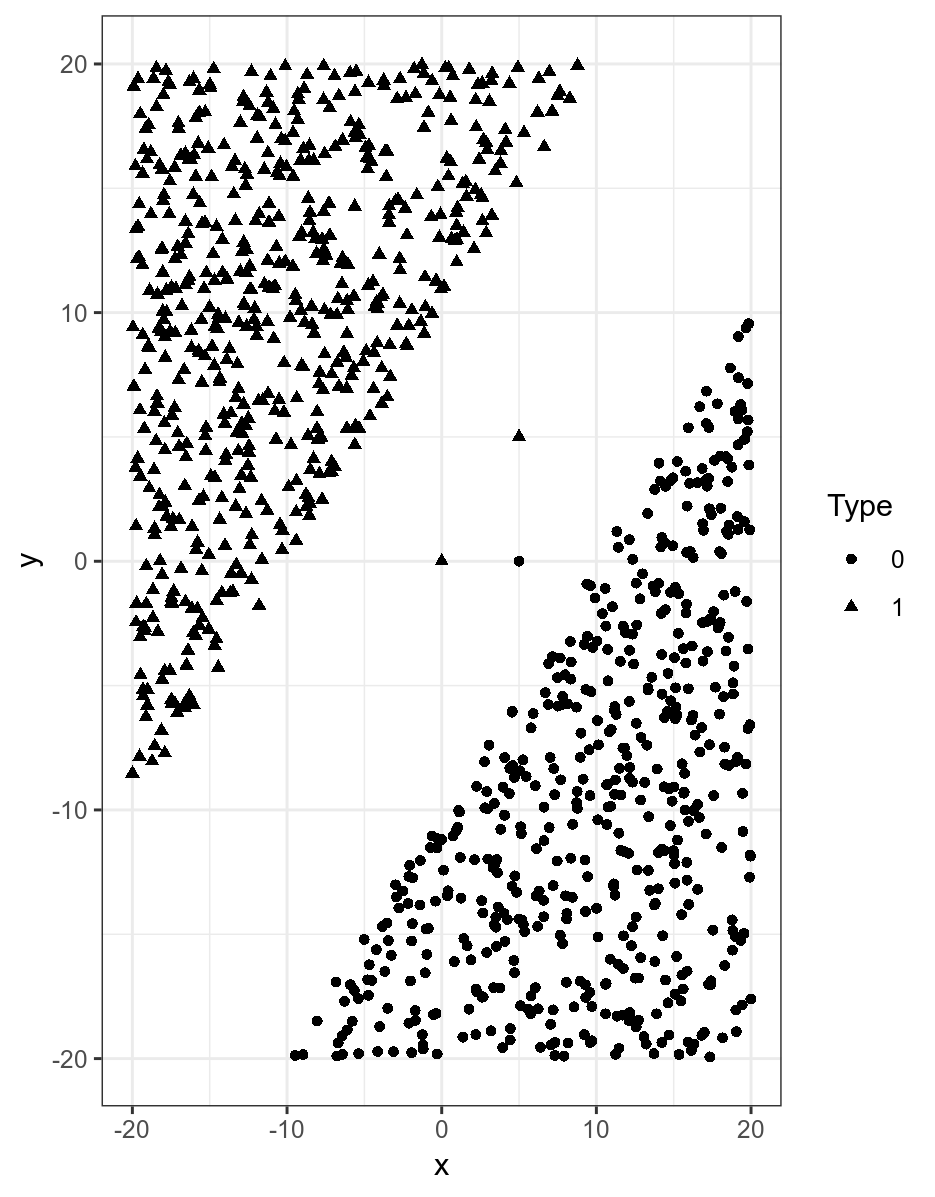
\includegraphics[scale=0.65]{R_plots/armada.png}
\end{center}
\end{minipage}


Целевая функция имеет вид:
\[
\min_{w, w_0} \frac{1}{2} w'w + C \sum_{i=1}^n \xi_i
\]

Уравнение разделяющей поверхности — $w'x = w_0$, уравнения краёв полосы: $w'x=w_0+1$ и $w'x=w_0-1$. Нарушителями считаются наблюдения, которые попали на нейтральную полосу или на чужую территорию. Здесь $\xi_i = |w| \cdot d_i$, где $d_i$ — длина «заступ» наблюдения за черту «своих».



\begin{enumerate}
\item Как пройдёт разделяющая полоса при $C=1$? Найдите $w$, $w_0$, и величины штрафов $\xi_i$.
\item Как пройдёт разделяющая полоса при $C=+\infty$? Найдите $w$, $w_0$, и величины штрафов $\xi_i$.
\end{enumerate}
\begin{sol}
\end{sol}
\end{problem}



\Closesolutionfile{solution_file}
